\RequirePackage{scrlfile}
\PreventPackageFromLoading{subfig}
\documentclass[a4paper,11pt]{article}

\usepackage{amsmath,amssymb,amsfonts}    % Typical maths resource packages
\usepackage[amsmath,amsthm,thmmarks]{ntheorem}
\usepackage{graphicx}                           % Packages to allow inclusion of graphics
\usepackage{svg}
\graphicspath{{./images/}{./images/background/}}
\usepackage[colorinlistoftodos, textsize=tiny]{todonotes}  
%\usepackage[colorinlistoftodos, textsize=tiny]{todonotes}   % todo notes
                          % For creating hyperlinks in cross references
%\usepackage[authoryear]{natbib}                 % literature reference style

%added
\usepackage[english]{babel}
\usepackage[utf8]{inputenc}
\usepackage[T1]{fontenc}
\usepackage{csquotes}
\usepackage[backend=biber,style=authoryear]{biblatex}
\addbibresource{Zotero.bib}
\usepackage[printonlyused]{acronym}
%% from tomepel/Technical_Book_DL
\def\layersep{2.5cm}
\usepackage{verbatim}
\usepackage[bf]{caption}
\usepackage{subcaption}
\usepackage{tabularx}
\usepackage{import}

\usepackage{enumitem}
\usepackage{gb4e}
% fixes gb4e - math collision
\noautomath

\usepackage{mathtools}
\DeclarePairedDelimiter{\abs}{\lvert}{\rvert}
\DeclarePairedDelimiter{\norm}{\lVert}{\rVert}


%\usepackage{ntheorem}
%\newtheorem{theorem}{Theorem}[Test]
\theoremstyle{nonumberplain}
\newtheorem{proposition}{Proposition}
\newtheorem{conjecture}{Conjecture}
%\theoremstyle{nonumberbreak}\theorembodyfont{\normalfont}\theoremsymbol{\ensuremath{\square}}
\theoremstyle{nonumberbreak}\theorembodyfont{\normalfont}
\newtheorem{reasoning}{Reasoning}
\newtheorem{rationale}{Rationale}
%\theoremstyle{nonumberplain}
%\theoremseparator{.}
%\theoremsymbol{\ensuremath{\Box}}
%\usepackage{pfsteps}


%added end

% -------------------------------
% --- some layout definitions ---
% -------------------------------

% define topline
\usepackage[automark]{scrpage2}
\pagestyle{scrheadings}
\automark{section}
\clearscrheadings
\ohead{\headmark}

% define citation style
%\bibliographystyle{ecta}

% define page size, margin size
\setlength{\headheight}{1.1\baselineskip}
\voffset=-2cm
\hoffset=-3cm
\textheight24cm
%\textwidth15.5cm
% just for todos:
\textwidth14.5cm
\setlength{\marginparwidth}{3.5cm} % make todonotes appear wider

\topmargin1cm
\oddsidemargin3cm
\evensidemargin3cm

% define line line spacing = 1.5
\renewcommand{\baselinestretch}{1.5}

% define second level for `itemizing'
\renewcommand{\labelitemii}{-}

\usepackage[colorlinks=true, allcolors=blue]{hyperref} 


% --------------------------------------
% --------------------------------------
% --------------------------------------
% --- the structure the tex document ---
% ---  (this our recommendation) -------
% frontmatter:
%   - titlepage (mandatory),
%   - acknowledgement,
%   - abstract,
%   - table of contents (mandatory),
%   - list of abbreviations (not mandatory),
%   - list of figures (not mandatory),
%   - list of tables  (not mandatory) .
%
% body of the thesis (the structure of the thesis body is not mandatory, but the list of literature is mandatory):
%   - introduction,
%   - methods,
%   - data,
%   - results,
%   - conclusion,
%   - literature (mandatory),
%   - appendix (figures, tables).
%
% last page:
%   - declaration of authorship (mandatory).
% --------------------------------------
% --------------------------------------
% --------------------------------------

\begin{document}

% -------------------------------
% --- frontmatter: Title page ---
% -------------------------------

%\thispagestyle{empty}
%\begin{center}

    {\Large{\bf Comparison of two semantic aware composition models for word embeddings and its relation to dependency type information}} \vspace{0.5cm}


    {\normalsize Student Research Paper submitted\\\vspace{0.5cm}
    to}\\\vspace{0.5cm}
    {\normalsize{\bf Prof. Ulf Leser}} \\\vspace{0.5cm}
    {\normalsize Humboldt-Universität zu Berlin \\
    Department of Computer Science \\
    Knowledge Management in Bioinformatics} \vspace{1cm}


    {\normalsize by \\\vspace{0.5cm}
    {\bf Arne Binder} \\
    (520999)} \vspace{1cm}


    %{\normalsize in partial fulfillment of the requirements \\
    %for the degree of \\
    %{\bf Bachelor/Master of Science} \\
    %{\normalsize Berlin, September 30, 2007}
    {\normalsize Berlin, \today}

\end{center}


%\pagenumbering{roman}   % define page number in roman style
\setcounter{page}{1}    % start page numbering

% -----------------------------
% --- frontmatter: Abstract ---
% -----------------------------
\newpage
\addcontentsline{toc}{section}{Expose}
\pagestyle{plain}
%\section*{Abstract}

\begin{center}
	\huge{Abstract} 
	\vspace{0.5cm}
	 
	\large{\bf{The impact of structural complexity on semantic aware composition of linguistic tokens}} 
	\vspace{0.5cm}

	%\hspace{10pt}
	% Author names and affiliations
	%\large
	by Arne Binder \\
	%\vspace{0.5cm}
	%\small  
	%$^1$) First affiliation\\
	%arthur.author@correspondence.email.com\\
	%$^2$) Second affiliation
\end{center}

%\hspace{10pt}
\vspace{0.5cm}
\normalsize

\acfp{VSM} for textual data lead to success in many \ac{NLP} tasks. Recently, prediction based word embedding models like word2vec %\autocite{mikolov_efficient_2013}
gained attention. These models build upon Distributional Semantics, i.e. a word is defined by its contexts, and scale up to billions of training tokens % \autocite{mikolov_distributed_2013}
resulting in robust embeddings for individual words. 
\acfp{CDSM} intend to create vector representations for sequences of tokens by composing word embeddings in a meaningful manner. However, it is up to debate which composition functions perform well for semantic tasks. \acp{RNN} produce appropriate results for short to medium length textual input on several semantic tasks \todo{CITATIONS}, but still suffer to handle long range dependencies and do not scale very well with text size\todo{CITATIONS}. 
\acp{RecNN} generalize \acp{RNN} by allowing arbitrary trees instead of sequences as input structure. in this means, the mean ...

In this work, we study the impact of structural complexity on semantic aware composition of linguistic tokens. Especially, we investigate if 

 generalizing  

models: tfidf, gru, sum, tree (gru + sum)
further inventions: following links (just for model==tree)
 

order aware processing to token embedding composition at sentence level by implementing (1) an averaging model and (2) a \ac{LSTM} based approach. Furthermore, we analyze the relation of order aware composition to syntactical information. We evaluate our models at the SICK relatedness prediction task.% \autocite{marelli_sick_2014}.

Our results underpin the thesis, that order aware processing is useful for semantic aware composition and subsumes syntactical information in most cases. However, there are instances of linguistic constructions in which syntactical information seems to be superior to order aware processing, namely in the presence of passive.


\clearpage

% -----------------------------
% --- frontmatter: Zusammenfassung ---
% -----------------------------
%\newpage
%\addcontentsline{toc}{section}{Zusammenfassung}
%\pagestyle{plain}
%
\begin{center}
	\huge{Zusammenfassung} 
	\vspace{0.5cm}
	
	\large{\bf{Comparison of two semantic aware composition models for word embeddings and its relation to dependency type information}} 
	\vspace{0.5cm}
	
	%\hspace{10pt}
	% Author names and affiliations
	%\large
	von Arne Binder \\
	%\vspace{0.5cm}
	%\small  
	%$^1$) First affiliation\\
	%arthur.author@correspondence.email.com\\
	%$^2$) Second affiliation
\end{center}

%\hspace{10pt}
\vspace{0.5cm}
\normalsize

CONTENT

%\clearpage

% ------------------------------------
% --- frontmatter: Acknowledgement ---
% ------------------------------------
%\newpage
%\pagestyle{plain}
%\pagenumbering{roman}   % define page number in roman style
%\setcounter{page}{1}    % start page numbering
%\section*{Acknowledgement}

I would like to thank



% -----------------------------
% --- frontmatter: Contents ---
% -----------------------------
%\newpage
%\tableofcontents
%\clearpage


% ----------------------------------------------------
% --- frontmatter: List of Abbreviations           ---
% ----------------------------------------------------
\newpage
\addcontentsline{toc}{section}{List of Abbreviations}
\ohead[]{LIST OF ABBREVIATIONS}
\section*{List of Abbreviations}

%\begin{tabular}{rp{0.2cm}lp{1cm}rp{0.2cm}l}
%    CPI     & &  Consumer Price Index   & & ETF     & &  Equity Traded Funds  \\
%    ETH     & &  Eat the Horse          & & XLM     & &  Xetra Liquidity
%\end{tabular}

\begin{acronym}
  \setlength{\parskip}{0ex}
  \setlength{\itemsep}{.8ex}
  
  %\acro{AFS}{Argument Facet Similarity}
  \acro{ANN}{Artificial Neural Network}
  \acro{AVG}{averaging}
  \acro{CDSM}{Compositional Distributional Semantics Model}
  \acro{CNN}{Convolutional Neural Network}
  \acro{DAN}{Deep Averaging Network}
  \acro{DG}{Dependency Grammar}
  \acro{DSM}{Distributional Semantics Model}
  \acro{FNN}{Feedforward Neural Network}
  \acro{FC}{fully connected layer}
  \acro{GRU}{Gated Recurrent Unit}
  \acro{LSA}{Latent Semantic Indexing}
  \acro{LSTM}{Long Short-Term Memory}
  \acro{IQR}{interquartile range}
  \acro{IR}{Information Retrieval}
  \acro{MSE}{Mean Squared Error}
  \acro{NLP}{Natural Language Processing}
  \acro{PMI}{Pointwise Mutual Information}
  \acro{PPMI}{Positive Pointwise Mutual Information}
  \acro{RecNN}{Recursive Neural Network}
  \acro{RNN}{Recurrent Neural Network}
  \acro{SGD}{Stochastic Gradient Descent}
  \acro{SGNS}{Skip-Gram model with Negative Sampling}
  \acro{STD}{standard deviation}
  \acro{STS}{Semantic Textual Similarity}
  \acro{SVD}{Singular Value Decomposition}
  \acro{TF-IDF}{term frequency-inverse document frequency}
  \acro{VSM}{Vector Space Model}
  
\end{acronym}



% ----------------------------------------------------
% --- frontmatter: List of Figures (not mandatory) ---
% ----------------------------------------------------
%\newpage
%\addcontentsline{toc}{section}{List of Figures}
%\ohead[]{\rightmark}
%\listoffigures



% ---------------------------------------------------
% --- frontmatter: List of Tables (not mandatory) ---
% ---------------------------------------------------
%\newpage
%\addcontentsline{toc}{section}{List of Tables}
%\listoftables



% -------------------------------
% --- main body of the thesis ---
% -------------------------------
\newpage
\pagestyle{plain}
%\setcounter{page}{1}    % start page numbering anew
\pagenumbering{arabic}  % page numbers in arabic style


%\section{Introduction} %\todo{(AG): Dreiteilung: (1) Researchkontext / Topaufgabe = 

Representations of textual content that are processable by computer algorithms form the basis for many applications that require to understand human utterances up to a certain extend. In this field, a common way is to transform textual data into high dimensional vector space representations, known as \ac{VSM}\autocite{salton_vector_1975}. These vector representations function as interface to a wide range of machine learning algorithms and leverage efficient approaches for many \ac{NLP} tasks like document retrieval \autocite{manning_introduction_2008}, text classification \autocite{sahami_bayesian_1998}, machine translation \autocite{wu_googles_2016} or argument clustering \autocite{boltuzic_identifying_2015}, among many others. However, the level of machine understanding is still not comparable to human performance\todo{AB:ref}. Recently, the Common Round\footnote{see \url{http://commonround.dfki.de/}} project \autocite{uszkoreit_common_2017} introduces a platform to facilitate large scale online debating with \ac{NLP} technologies. The authors define aggregation of the semantic content of debates as one of their major objectives which they intend to achieve by clustering similar arguments. That approach requires a scalable, semantically consistent similarity measure for text, emphasizing the need for a well structured semantic vector space. 

Frameworks like word2vec \autocite{mikolov_distributed_2013} or glove \autocite{pennington_glove_2014} lead to success in many \ac{NLP} tasks by producing dense vector representations for single words. The cosine distance of these so called \textit{word embeddings} enables a semantically consistent similarity measure for word tokens. \acp{CDSM} introduced by \textcite{clark_compositional_2008} exploit this by combining sequences of word embeddings in a functional manner to produce vector representations of arbitrary textual utterances that are to a degree semantical consistent. However, there is an ongoing debate how to effectively combine word embeddings for gaining better performance. Several approaches build on simple summation or averaging \autocite{habernal_exploiting_2015,boltuzic_identifying_2015,misra_measuring_2016}. Then again, \Textcite{misra_measuring_2016} state that averaging all word embeddings may lose too much information in long sentences. \Textcite{wang_comparison_2017} present an overview of different embedding composition models for phrase representations. They conclude that the recurrent \ac{LSTM} model \autocite{hochreiter_long_1997} that processes tokens in order just slightly outperforms the additive, order unaware baseline model in this task. \Textcite{tai_improved_2015} introduced another level of complexity by presenting the recursive TreeLSTM model. This model further reduces the vanishing gradient problem as compared to recurrent models by shortening the average distance of entities in the computation graph. The authors use dependency parse trees to construct the neural model and present promising results for the SICK phrase relatedness task\footnote{The SICK corpus \autocite{marelli_sick_2014} contains $\sim$10.000 similarity scored sentence pairs. The system by \Textcite{tai_improved_2015} achieved a Pearson's $r$ of 0.8676 when predicting the similarities.}. 

Recently, \Textcite{mueller_siamese_2016} presented a simple \ac{LSTM} based approach. Despite it does not require any syntactical information as dependency structure, it still outperforms the TreeLSTM model by \textcite{tai_improved_2015}. Furthermore, \Textcite{iyyer_deep_2015} introduces the \ac{DAN} that performs well on several semantic tasks even without exploiting any ordering information of the tokens. It seems to be an open question what kind of structural information impacts semantic aware processing to what degree.



%clustering similar arguments (ok) (2) Was gibt es schon.  Welche Probleme gibt es schon? Motivation: z.B. aus Misra: "averaging word2vec embeddings for each
%word may lose too much information in long sentences."(3) Mein wissenschaftlicher Beitrag ()}

%Large online debates\todo{UL:add examples, numbers} contain redundant arguments and therefore hinder efficient debating.
%To tackle this problem, \Textcite{boltuzic_identifying_2015} proposed to cluster similar arguments and filter only the most representative ones.\todo{UL:explain further (intention?)} The Common Round\footnote{see \url{http://commonround.dfki.de/}} project \autocite{uszkoreit_common_2017} introduces a platform to facilitate large scale online debating with \ac{NLP} technologies. The authors define the aggregation of the semantic content of debates as one of their major objectives which they intend to achieve by clustering similar arguments.
%Moreover, \Textcite{misra_measuring_2016} define the \ac{AFS} task as the recognition of the semantic similarity of two sentential arguments.\todo{AB:move away from arguments as motivation!}

%\vspace{11pt}
%\bigskip
%\noindent
%To achieve these\todo{UL:more precise!} goals, a semantically consistent similarity measure for arguments is necessary. Frameworks like word2vec \autocite{mikolov_distributed_2013} or glove \autocite{pennington_glove_2014} lead to success in many \ac{NLP} tasks by producing dense embedding vectors for single words. The cosine distance of these word embeddings enables a semantically consistent similarity measure for word tokens. Building on this, \Textcite{habernal_exploiting_2015,boltuzic_identifying_2015,misra_measuring_2016} use summed or averaged word embeddings for argument similarity measures. 
%However, \Textcite{misra_measuring_2016} state that averaging all word embeddings may lose too much information in long sentences. \Textcite{wang_comparison_2017} present an overview of different embedding composition models for phrase representations. They conclude that the recurrent \ac{LSTM} model \autocite{hochreiter_long_1997} just slightly outperforms the additive baseline model in this task. \Textcite{tai_improved_2015} introduced the recursive TreeLSTM model which further reduced the vanishing gradient problem as compared to recurrent models by shortening the average distance of entities in the computation graph. The authors use dependency parse trees to construct the neural model and present promising results for the SICK phrase relatedness task\footnote{The SICK corpus \autocite{marelli_sick_2014} contains $\sim$10.000 similarity scored sentence pairs. The system by \Textcite{tai_improved_2015} achieved a Pearson's $r$ of 0.8676 when predicting the similarities.}. 

%\vspace{11pt}
%\bigskip
%\noindent
%However, these models\todo{UL:specify!} are applied to sentences, but not yet to multi-sentence arguments or paragraphs. Additionally, their\todo{UL:specify!}  approach does not use dependency edge type information such as 'nsubj' (nominal subject) or 'prep' (preposition).

\subsection{Objective}
In this work we examine what degree of semantic awareness is achievable with two different, existing embedding composition models, that vary in complexity, when applied to sentences (Section~\ref{sec:approach}).%\todo{UL:clarify sentence level vs. super-sentence level mismatch}. 
We regard composition of word embeddings as semantic aware if it yields a distance measure that matches human intuition. Furthermore, we study the impact of providing syntactical data for the respective architectures.
%Furthermore, our goal is to provide access to the rapid implementation of different neural network topologies including \acp{RecNN} for semantically aware composition.

\subsection{Approach}
\label{sec:approach}
To achieve these goals we implement the following: (a) an averaging model, and (b) a neural sequence model. We evaluate the semantic awareness with the SICK \ac{STS} challenge \autocite{marelli_sick_2014} and compare the model performances against a \acs{TF-IDF} baseline.

%To prepare for rapid comparison with various neural models, we use the Tensorflow Fold\footnote{see \url{https://github.com/tensorflow/fold}} framework \autocite{looks_deep_2017} for implementation. It allows fast training of neural networks with dynamic computation graphs, i.e. networks whose structure depends on the data that is fed during training. Moreover, it is based on Tensorflow\footnote{see \url{www.tensorflow.org}} which is widely used as a deep learning framework.

%Furthermore, we tackle the data sparsity problem by examining pre-training capabilities 

%\subsection*{Model details}
As neural sequence model, we use an approach based on \Textcite{mueller_siamese_2016} due to its simplicity. It consists of one LSTM as composition model which is applied to two input sentences and uses the Manhattan metric as distance measure. Nevertheless, the authors report a Pearson's $r$ of 0.8822 for the SICK challenge. In our averaging setting, every word embedding is mapped by one identical, non-linear transformation before their aggregation.

We analyze the effect of syntactical information by optionally appending one-hot encoded dependency type data to the token embedding vectors. 

%\subsection*{Dataset enlargement}
%One major drawback of the SICK corpus is its small size. We will use pre-training with paraphrase data from the PPDB\footnote{see \url{http://paraphrase.org}} corpus \autocite{ganitkevitch_ppdb_2013} and evaluate its effect to the model performances. In its smallest, most accurate version the phrasal subset of the corpus contains 1,530,812 pairs of short phrase snippets like ('\texttt{maintain international peace and}', '\texttt{maintaining world peace and}'). We treat these pairs as similar and extend the dataset with artificially generated negative samples where the two phrases are randomly sampled from the corpus.

%\newpage
%\section{Theoretical Background}



\if false
===OLD SRP CONTENT===


This chapter provides an overview of basic concepts regarding semantic aware vector space representations and neural machine learning. Furthermore, we briefly introduce linguistic dependency types.

\subsection{Evaluation of Semantic Awareness} \label{subsec:eval_semantic_awareness}
%sahlgren_distributional_2008
Following the Distributional Hypothesis \autocite{harris_distributional_1954}, that linguistic items with similar contexts have similar meanings, it should be possible to construct a conceptional space in a way, that distances of concepts follow human intuition.
%a conceptional space should be arranged in a way, that distances of concepts follow the human intuition. By doing so, the meaning of these concepts should be as expected as by humans. 
\acfp{DSM} \autocite{landauer_solution_1997,schutze_automatic_1998} are approaches that implement this thesis.

With semantic awareness we describe the property of how much meaning a representational space is able to preserve with respect to the space of origin, textual natural language. Furthermore, the theoretical state of being semantic aware references the maximal achievable semantic awareness, i.e. conveying the same meaning as the origin of the representation.

With regard to the Distributional Hypothesis semantic awareness can be measured by the correlation of the distances between different concepts in the representational space and the distances between its representations in the original space. Although the concept of \textit{distance} seems to be more intuitive in the context of representational spaces, its inverse, the concept of \textit{similarity}, commonly serves as base of comparison.  

Given similarity measures that map from both spaces into the same space $X \subseteq \mathbb{R}$, we can borrow the task of \textit{similarity prediction} for evaluation of semantic awareness when using \textit{semantic relatedness} as underlying similarity metric of $X$. With the concept of semantic relatedness we refer to the interpretation by \textcite{budanitsky_evaluating_2006}: \textit{linked by any kind of lexical or functional association}. \textcite{resnik_semantic_1999} visualizes this concept by contrasting it with \textit{semantic similarity}. The authors state that "car" and "gasoline" are related, but not semantically similar, whereas "car" and "bicycle" are semantic related \textit{and} similar. Thus, semantic similarity covers only a subset of semantic relatedness and captures relations like synonymy or hypernymy while semantic relatedness further captures antonomy, meronymy and others.

The capability of predicting this kind of similarity by using an internal representation requires by definition some degree of semantic awareness. We are going to evaluate to which extent that might be the case in different scenarios.% for different composition methods.

%The distance should not be interpreted as the inverse of semantic similarity, but of semantic \textit{relatedness}. As \textcite{budanitsky_evaluating_2006} highlight, semantic similarity is a specific kind of relatedness (the same applies to antonymy, entailment and others). Therefore, measuring semantic relatedness covers semantical awareness in a more general and accurate way \todo{UL:evidence? Ref!} than other textual comprehension tasks like recognizing textual entailment (RTE)\todo{UL:Ref}, for instance. 

%When we use the sole term \textit{similarity} in the following, we do not reference semantic similarity, but semantic relatedness, like in the common literature about semantic \ac{NLP}.     

\subsubsection{Similarity Prediction}
%In the context of \ac{NLP} 
The task of Similarity Prediction can be framed as to predict a score given two entities of a conceptional space, where higher scores represent higher degrees of similarity between them. In the context of \ac{NLP} these entities are linguistic units such as words, phrases, sentences or documents. The score can include different granularities of similarity, ranging from binary classification, e.g. in the case of Paraphrase Detection\footnote{Paraphrase Detection is the task of identifying if two phrases paraphrase each other.}, weighted aggregation of multi-label classification results, e.g. for instances of discrete %Likert-scaled 
questionnaire data, to regression with continuous scores. 
%Considering its more general nature and the availability of 5-point Likert-scored evaluation data, we will focus on Similarity Prediction as regression task.
%With regard to natural language, \Textcite{agirre_semeval-2012_2012} defines \acf{STS} as the measure for the degree of semantic equivalence \todo{UL: relatedness?} between two texts.\todo{UL: sinnlos, AB: rework or move}

We will focus on Similarity Prediction as regression task. Semantic Relatedness of arbitrary\footnote{The composition is surely constrained by grammar, linguistic performance and other criteria, but this term is in favor of the tremendous variability of natural language.} composed textual entities is no binary phenomena. Otherwise the entity space would disintegrate into distinct clusters each containing entities interpreted as identical. %\todo{UL: the following is unnecessary}As semantic relatedness is defined about \textit{any} kind of lexical or functional association, it is expected that any entity is semantical related with the majority of the entities in the space in a transitively manner allowing only the trivial solution, precisely, that all entities are identical with respect to the similarity. The compensation of this fact increases the amount of necessary data to approximate the real behavior. Furthermore, modeling Similarity Prediction as regression is straightforward compared to aggregation of multi-classification output.  

\subsubsection{Evaluation Measures} \label{sec:eval_measures}
Common measures for evaluation of regression estimators are \textit{\acl{MSE}} \autocite[see][]{lehmann_theory_1998}, \textit{Pearson correlation coefficient} \autocite{pearson_note_1895} and \textit{Spearman's rank correlation coefficient} \autocite{spearman_proof_1904}.

The \acf{MSE} measures the deviation of the predicted values to the correct ones. It incorporates the variance and the bias of the estimator. A value of zero denotes a perfect estimator and larger values indicate lower estimator performance. Given $n$ predictions $Y$ and corresponding correct values $X$, the \ac{MSE} is defined as follows:
\begin{equation} \label{eq:eval_measure_mse}
MSE = \frac{1}{n}\displaystyle\sum_{i=1}^{n} (Y_i - X_i)^2
\end{equation}

The Pearson correlation coefficient (Pearson's $r$) expresses the degree of linear correlation of two variables. It is the covariance of the variables normalized by their standard deviations. It ranges from $-1$, denoting perfect negative correlation, to $1$, denoting perfect positive correlation. A value of zero expresses that the two variables do not correlate at all. Therefore, higher values above zero indicate better estimator performance. Given $X$ and $Y$, Pearson's $r$ is defined as:
\begin{equation}
r = \frac{\sum_{i=1}^{n}(X_i - \overline{X})(Y_i - \overline{Y})}{\sqrt{\sum_{i=1}^{n}(X_i - \overline{X})^2 \cdot \sum_{i=1}^{n}(Y_i - \overline{Y})^2}} = \frac{Cov(X, Y)}{\sigma(X) \sigma(Y)},
\end{equation}
where $\overline{X}$ is the empirical mean of $X$, $Cov(X, Y)$ is the empirical covariance of $X$ and $Y$, and $\sigma(X)$ is the empirical standard deviation.
%\begin{equation}
%\overline{X} = \frac{1}{n}\displaystyle\sum_{i=1}^{n} X_i;\quad %\text{analogously } \overline{Y}. 
%\end{equation}

Spearman's rank correlation coefficient (Spearman's $\rho$) serves as another correlation based measure, which does not assume linear dependence between $X$ and $Y$. Hence, it is more robust regarding outliers. Spearman's $\rho$ can be interpreted as special case of Pearson's $r$ where the data is converted into ranks before calculation of Pearson's $r$. Given $X$ and $Y$, Spearman's $\rho$ is defined as:
\begin{equation}
\rho = \frac{\sum_{i=1}^{n}(rg(X)_i - \overline{rg(X)})(rg(Y)_i - \overline{rg(Y)})}{\sqrt{\sum_{i=1}^{n}(rg(X)_i - \overline{rg(X)})^2 \cdot \sum_{i=1}^{n}(rg(Y)_i - \overline{rg(Y)})^2}} = \frac{Cov({rg(X)}, {rg(Y)})}{\sigma({rg(X)})\sigma({rg(Y)})},
\end{equation}
where $rg(X)$ are the ranks of $X$. 

%\begin{itemize}[label=]
%\item $rg(X_i)$ is the rank of $X_i$,
%\item $\overline{rg}_X$ is the mean of the ranks of $X$,
%\item $\sigma_{{rg}_X}$ is the standard deviation of the ranks of $X$, and
%\item $Cov({rg}_X, {rg}_Y)$ is the covariance of the ranks of $X$ and $Y$.
%\end{itemize}

\subsection{Artificial Neural Networks}
An \ac{ANN} is a machine learning model where input vectors are mapped to predictions by successive application of computational \textit{layers} \autocite{rumelhart_parallel_1986}. Each layer is a differentiable function $l^{(i)}: \mathbb{R}^{n^{(i-1)}} \mapsto \mathbb{R}^{n^{(i)}}$, with $n^{(i)}$ denoting the size of the $i$-th layer. %input vector for the $i$-th layer, its \textit{layer size}. 
The arrangement of layers form the network graph, which is (in most cases) a directed graph defining the specific network architecture. Provided adequate training data, \ac{ANN}s can be trained efficiently with gradient descent based optimization algorithms\todo{UL:ref}. In the next sections we will describe some popular architectures and important components of \ac{ANN}s. 

\subsubsection{Feedforward Networks}
The simplest class of \ac{ANN}s are \acl{FNN}s (\acs{FNN}s) that emerged from multilayer Perceptrons \autocite{rosenblatt_perceptron_1958}. Their network architecture forms an acyclic graph and is defined by $f^{FNN}(v) = (l^{(N)} \circ ... \circ l^{(i)} \circ ... \circ l^{(1)})(v)$ where $N$ is the total amount of layers. The $N$-th layer is called \textit{output layer}, all other layers are \textit{hidden layers}. In addition, a virtual \textit{input layer} models the input. Figure~\ref{fig:1} \autocite{epelbaum_deep_2017} shows such a structure. 

%% graphic taken from tomepel/Technical_Book_DL
\begin{figure}[h]
\begin{center}
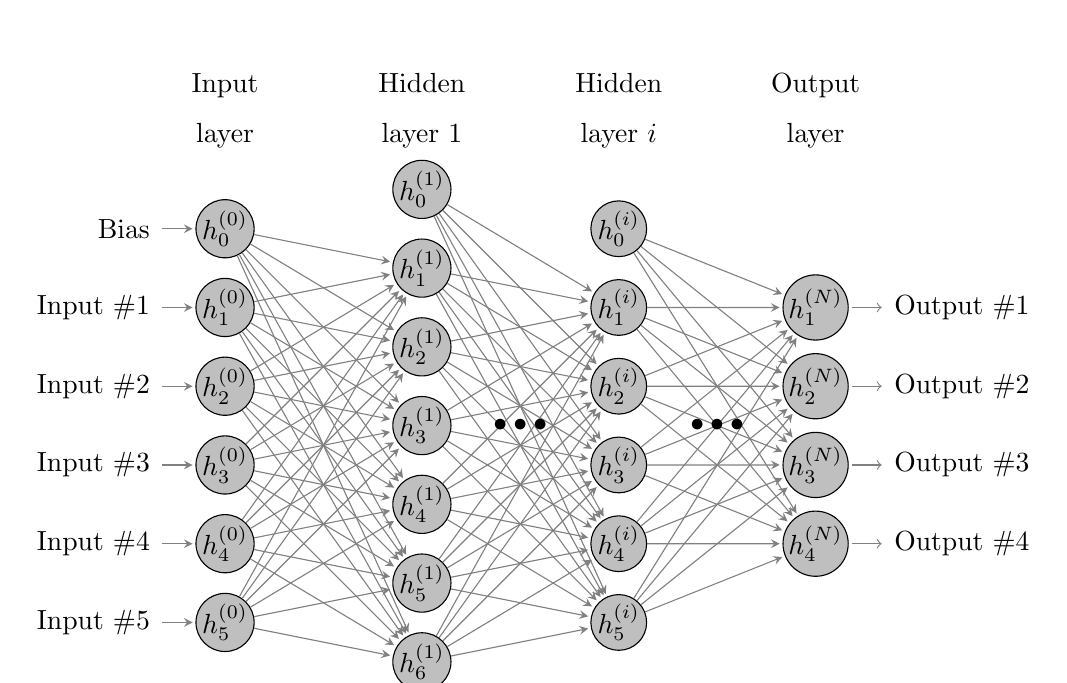
\begin{tikzpicture}[shorten >=1pt,-stealth,draw=black!50, node distance=\layersep]
    \tikzstyle{every pin edge}=[stealth-,shorten <=1pt]
    \tikzstyle{neuron}=[circle,draw=black,fill=black!25,minimum size=17pt,inner sep=0pt]
    \tikzstyle{input neuron}=[neuron, fill=gray!50];
    \tikzstyle{output neuron}=[neuron, fill=gray!50];
    \tikzstyle{hidden neuron}=[neuron, fill=gray!50];
    \tikzstyle{annot} = [text width=4em, text centered]

    % Draw the input layer nodes
    \foreach \name / \y in {1}
       	\pgfmathtruncatemacro{\m}{int(\y-1)}
    % This is the same as writing \foreach \name / \y in {1/1,2/2,3/3,4/4}
        \node[input neuron, pin=left:Bias] (I-\name) at (0,-\y) {$h_{\m}^{(0)}$};


    \foreach \name / \y in {2,...,6}
       	\pgfmathtruncatemacro{\m}{int(\y-1)}
    % This is the same as writing \foreach \name / \y in {1/1,2/2,3/3,4/4}
        \node[input neuron, pin=left:Input \#\m] (I-\name) at (0,-\y) {$h_{\m}^{(0)}$};

    % Draw the hidden layer 1 nodes
    \foreach \name / \y in {1,...,7}
    	\pgfmathtruncatemacro{\m}{int(\y-1)}
        \path[yshift=0.5cm]
            node[hidden neuron] (H1-\name) at (\layersep,-\y cm) {$h_{\m}^{(1)}$};

    % Draw the hidden layer i node
    \foreach \name / \y in {1,...,6}
        \pgfmathtruncatemacro{\m}{int(\y-1)}
        \path[yshift=0.0cm]
            node[hidden neuron] (H2-\name) at (2*\layersep,-\y cm) {$h_{\m}^{(i)}$};

    % Draw the output layer node
    \foreach \name / \y in {1,...,4}
        \path[yshift=-1.0cm]
    node[output neuron,pin={[pin edge={->}]right:Output \#\y}] (O-\name) at (3*\layersep,-\y cm) {$h_{\y}^{(N)}$};

    % Connect every node in the input layer with every node in the
    % hidden layer.
    \foreach \source in {1,...,6}
        \foreach \dest in {2,...,7}
            \path (I-\source) edge (H1-\dest);

     \foreach \source in {1,...,7}
       \foreach \dest in {2,...,6}
           \path (H1-\source) edge (H2-\dest);

    % Connect every node in the hidden layer with the output layer
    \foreach \source in {1,...,6}
       \foreach \dest in {1,...,4}
          \path (H2-\source) edge (O-\dest);

    % Annotate the layers
    \node[annot,above of=H1-1, node distance=1cm] (hl) {Hidden layer 1};
    \node[annot,left of=hl] {Input layer};
    \node[annot,right of=hl] (hm) {Hidden layer $i$};
    \node[annot,right of=hm] {Output layer};

    \node at ((1.5*\layersep,-3.5 cm) {$\bullet\bullet\bullet$};
    \node at ((2.5*\layersep,-3.5 cm) {$\bullet\bullet\bullet$};
\end{tikzpicture}
\caption{\label{fig:1}Neural Network with $N+1$ layers ($N-1$ hidden layers).}
\end{center}
\end{figure}

There exists a diverse landscape of different types of layers. A common structure is the \ac{FC}. It connects every node from the previous layer with every node from the current one in the form of a weighted sum \todo{UL: Sprung von "connection" zu "aggregation"}. Hence, it calculates an affine transformation of its input. Usually a layer $l^{(i)}$ is parametrized by $\theta^{(i)}$, e.g. a set of \textit{weights} and \textit{biases}. In this manner, a \ac{FC} can be defined as:
\begin{equation}
l^{FC}(v;\theta^{(i)}) = w^{(i)}v+b^{(i)} 
\end{equation}
where $w^{(i)} \in \mathbb{R}^{n^{(i)} \times n^{(i-1)}}$, $b^{(i)} \in \mathbb{R}^{n^{(i)}}$ and $\theta^{(i)}=\{w^{(i)}, b^{(i)}\}$. 

\subsubsection{Activation Functions}
The \ac{FNN} described so far is capable of modeling linear mappings only. To enable non-linearity, different non-linear activation functions can be applied element-wise to the individual layer outputs. A prominent instance is the \textit{sigmoid} function that takes a real-valued input and "squashes" it to range between 0 and 1. Therefore, it is used to model Bernoulli-Distributions. It is defined as:
\begin{equation}
\sigma(v_i)=\frac{1}{1+e^{-v_i}}
\end{equation}
\todo{UL: what is "x"? explain!}
The \textit{hyperbolic tangent} is another strictly increasing, non-linear activation function, but maps into the range between -1 and 1:
\begin{equation}
\tanh(v_i)=\frac{1-e^{-2v_i}}{1+e^{-2v_i}}=2\sigma(2v_i)-1
\end{equation}

Finally, the \textit{softmax} function can be used to model discrete probability distributions, e.g. for classification tasks. In contrast to the previous activation functions it is not element wise independent, since it applies normalization across all input elements to guarantee that its result follow the probability distribution conditions. For an input vector $x$ with entries $x_i$ it is defined as:
\begin{equation}
softmax(v_i) = \frac{e^{v_i}}{\sum\limits_{v_j \in v}e^{v_j}} 
\end{equation}

\subsubsection{\acl{RNN}s} \label{subsec:rnn}
\acl{RNN}s (\acs{RNN}s) introduced by \textcite{hopfield_neural_1982} are \ac{ANN}s that are capable of processing arbitrary long sequences when feeding them stepwise into the network. Additionally, they can access information from any previous step and, hence, process the new data conditioned by historical data. This is possible via a feedback loop in a \textit{recurrent layer}. Given a sequence of $\tau$-sized vectors $v^{(1)}, ..., v^{(\eta)}$ the $t$-th output $h^{(t)}$ of a recurrent layer $l^{RNN}$ is defined as:
\begin{equation} \label{eq:rnn}
h^{(t)} = l^{RNN}(v^{(t)};\theta) = g(v^{(t)}; h^{(t-1)};\theta)
\end{equation}
where $k, \vartheta \in \mathbb{N}$, $k$ is the inner state size and $g$ is the \ac{RNN} cell \todo{UL: define "cell"} function with $g:(\mathbb{R}^\tau; \mathbb{R}^k; \mathbb{R}^\vartheta) \mapsto \mathbb{R}^k$.

The \acf{LSTM} \autocite{hochreiter_long_1997} is a prominent \ac{RNN}. It is a \textit{gated} \ac{RNN}, meaning its cell function $g^{LSTM}$ consists of multiple interconnected gating functions that model a dedicated cell state $\tilde{c}$ (Equation~\ref{eq:lstm_interm}). \ac{LSTM}s tackle one major drawback of the \ac{RNN} architecture, namely the vanishing gradient problem that occurs when training with long sequences\todo{UL:ref}. Without gating, repeated application of \ac{RNN} cell \todo{UL: finding (??)} to the elements of a sequence often leads to exponential decrease of the calculated gradients because common activation functions produce gradients lesser 1 that are multiplied according to the chain rule. That effect practically hinders the network to use long-distance information. Section~\ref{subsec:gradient_optimization} explains the exact role of gradients in neural network training.

The different gates \todo{UL:add figure!} of the \ac{LSTM} are responsible for deciding what information should be forgotten ($g_f$), which new information will be added ($g_i$) and, finally, which information from the cell state $\tilde{c}$ will be presented as output ($g_o$):

\begin{equation} \label{eq:lstm_interm}
\begin{split}
g_f^{(t)} & = \sigma(l^{FC}([\tilde{h}^{(t-1)}, v^{(t)}]; \theta^{(f)})) \\
g_i^{(t)} & = \sigma(l^{FC}([\tilde{h}^{(t-1)}, v^{(t)}]; \theta^{(i)})) \\
g_o^{(t)} & = \sigma(l^{FC}([\tilde{h}^{(t-1)}, v^{(t)}]; \theta^{(o)})) \\
c^{(t)} & = tanh(l^{FC}([h^{(t-1)}, v^{(t)}]; \theta^{(c)})) \\
\tilde{c}^{(t)} & = g_f^{(t)} \odot \tilde{c}^{(t-1)} + g_i^{(t)} \odot \tilde{c}^{(t-1)} \\
\tilde{h}^{(t)} & = g_o^{(t)} \odot tanh(\tilde{c}^{(t)})
\end{split}
\end{equation}
and finally
\begin{equation} \label{eq:lstm}
g^{LSTM}(v^{(t)};[\tilde{c}^{(t-1)}, \tilde{h}^{(t-1)}]) = [\tilde{c}^{(t)}, \tilde{h}^{(t)}]
\end{equation}
where $[a, b]$ is the concatenation of the vectors $a$ and $b$, and $a \odot b$ denotes their element-wise  product (Hadamard product). We omit the parameter set $\theta^{LSTM} = \{\theta^{(f)}, \theta^{(i)}, \theta^{(o)}, \theta^{(c)}\}$ for better readability.

\subsection{Supervised Training of ANNs}
%In this section we describe the optimization procedure for \acl{ANN}s, e.g their training. 
Supervised training of an \ac{ANN} model $f$ parametrized by $\theta$ takes a set $\Omega$ of input-output training tuples $(x,y)$ for granted and tries to find instantiations of $\theta$ in the manner that $f(x;\theta) = \hat{y} \approx y, \forall (x,y) \in \Omega$ \autocite{mohri_foundations_2012}. In the context of \ac{ANN}s, one usually uses a \textit{cost function} $J$ that quantifies the deviation of $\hat{y}$ from $y$, thus $J$ is used to guide the parameter adjustment via gradient-based optimization to minimize this cost.%\todo{AB: rework (see J below)}

\subsubsection{Cost Function}
\label{subsec:cost_function}
The cost function, or \textit{loss function}, most commonly used for regression tasks is \acf{MSE} as described in section~\ref{sec:eval_measures}, because it yields the maximum likelihood of $y$ and $\hat{y}$ if the error is normally distributed and because it is efficient to calculate. We reformulate equation~\eqref{eq:eval_measure_mse} to fit into our needs:
\begin{equation}
J^{MSE}_\Omega(\theta) = \frac{1}{n}\sum_{i=0}^{n-1}\sum_{j=0}^{\iota-1}(y_{ij}-\hat{y}_{ij})^2 \label{eq:j_mse}
\end{equation}
where $n$ is the amount of tuples $(x_i, y_i)$ in $\Omega$ and $\hat{y}_i = f(x_i;\theta)$ with $y_i, \hat{y_i} \in \mathbb{R}^\iota$. %Note that, although the cost function depends on the training samples, these are considered to be fixed. 

\subsubsection{Gradient-based Optimization} \label{subsec:gradient_optimization}
If the loss function $J_\Omega$ is differentiable, in theory it would be possible to calculate its global minimum $\theta^*$ analytically. However, in practice this is infeasible due to the number of parameters in $\theta$ that can be in the order of millions. For instance, the VGG network \autocite{simonyan_very_2014} uses up to 144 million trainable weights for image recognition tasks.
%that requires to determine the gradients $\triangledown J_\Omega$ according to all entries in $\Omega$ which is infeasible for large training sets.

Gradient-based optimization \todo{UL: ref} tackles this problem by shifting the parameters $\theta$ stepwise in the negative direction of its gradients $\triangledown J_\Omega$. By definition of gradients, an infinitesimal displacement of $\theta$ in this direction decreases $J_\Omega(\theta)$. Hence, we select the parameters for the next optimization step $\theta'$:
\begin{equation}
\theta' = \theta - \alpha\triangledown J_\Omega(\theta)
\end{equation}
where $\alpha$ is the chosen step size, or \textit{learning rate}, that has to be sufficiently small. On the other hand, it is unfavorable to choose a step size too small because that increases convergence time, meaning it slows down training. Also different approaches exist that apply dynamical sized stepping like \textit{Momentum} \autocite{polyak_methods_1964}, which takes previous parameter updates into account, or \textit{AdaDelta} \autocite{zeiler_adadelta_2012} that tracks individual learning rates for the parameters in $\theta$. ADAM \autocite{kingma_adam_2014} is another robust method to guide the parameter optimization by keeping track of the gradients and its square roots.   

As equation \eqref{eq:j_mse} states, one update step requires summation over all training examples in $\Omega$, so it is an $O(n)$ operation. %\todo{AB:really? not higher?}. 
Hence, with large training sets calculation of $\triangledown J_\Omega(\theta)$ for every step becomes infeasible. \ac{SGD} \todo{UL: ref} addresses this problem by randomly partitioning $\Omega$ into subsets $\Omega^P_i$ % of size $n^B$ \todo{UL: what is B?} 
that are used successively to calculate new parameter sets $\theta'$. Exhausting all $\Omega^P_i$, also referred to as \textit{(mini-)batches}, of a certain partition $\Omega^P$ is called finishing an \textit{epoch}. This approach stochastically approximates the calculation of $\triangledown J_\Omega(\theta)$.

Finally, we describe the core algorithm that enables gradient-based training of \ac{ANN}s, namely \textit{Backpropagation} \autocite{rumelhart_learning_1988}. It uses dynamic programming for efficient calculation of the gradients through the different layers by exploiting their interconnectivity as present in common \ac{ANN}s. As stated before, an \ac{ANN} $f$ can be represented as a composition of layer functions $l^{(i)}$ with $f(v) = (l^{(N)} \circ ... \circ l^{(i)} \circ ... \circ l^{(1)})(v)$ and $l^{(i)}(v^{(i)}) = v^{(i+1)}$. Hence, the \textit{chain rule} of gradient computation defines the derivatives for two successive layers as:  
\begin{align}
  \frac{dv^{(i+2)}}{dv^{(i)}} & = \frac{dv^{(i+2)}}{dv^{(i+1)}}\frac{dv^{(i+1)}}{dv^{(i)}} \label{eq:chain_1}\\
    & = l^{(i+1)'}(v^{(i+1)})l^{(i)'}(v^{(i)}) \label{eq:chain_2}\\
    & = l^{(i+1)'}(l^{(i)}(v^{(i)}))l^{(i)'}(v^{(i)})  \label{eq:chain_3}
\end{align}
$v^{(i)}$ occurs several times in equation \eqref{eq:chain_3}. Furthermore, as shown in \eqref{eq:chain_1} $\frac{dv^{(i+2)}}{dv^{(i)}}$ depends on $\frac{dv^{(i+2)}}{dv^{(i+1)}}$ immediately. Backpropagation exploits these redundancies by successively calculating all $v^{(i)}$ in a \textit{forward pass}. Then, it calculates all gradients in reverse order while reusing intermediate results in a \textit{backwards pass}. By doing so, the algorithm reduces the complexity from exponential, considering a naive approach, to linear with regard to the edge count of the network graph.

\subsection{A Model for Semantic Relatedness Prediction}
We divide semantic relatedness prediction with regard to textual inputs into (1) transformation of the inputs into vector space representations and 
%similarity measure application. 
(2) similarity calculation in this embedding space.
%Similarity prediction with regard to textual inputs can be divided into transformation of the inputs into vector space representations and similarity measure application.

\subsubsection{Vector Space Embeddings}
We define \textit{embeddings} of documents, words or other linguistically motivated units as vector representations that are to a degree semantically aware. \textit{Embedding models} are transformations that map these units into an \textit{embedding space}.

Because of the relevance of embedding models for many \ac{NLP} tasks, a diverse landscape of different approaches has evolved\todo{UL: ref (survey)}. In the following, we distinguish traditional document embedding approaches from composition based models. By traditional approaches we refer to models which process sequences of opaque tokens and directly produce embeddings for these sequences \autocite[see][for an exhaustive study]{turney_frequency_2010}, whereby composition based models \autocite{clark_compositional_2008,grefenstette_experimental_2011} initially embed each token independently and compose these token embeddings into a final vector space representation.

\subsubsection{Traditional Document Embeddings}
\label{subsec:doc_embedding}
%\todo{AB:name Vector Space Models!} XXX READ: \autocite{turney_frequency_2010}
%As we focus on distributional semantics, we can outline some common features for traditional document embedding models. 
\acfp{VSM} \autocite{turney_frequency_2010} \todo{UL: better: original ref} build upon occurrences of terms $T$ within certain contexts $C$. For example, a word can occur as term in a document, i.e. its context, or not. In \acp{VSM} contexts are expressed in means of terms that occur with these. Thus, these models are instances of \acp{DSM} (Section~\ref{subsec:eval_semantic_awareness}).  We define $T = \{t_1, ..., t_m\}$ as finite set of opaque symbols with $m = |T|$ and the set of contexts $C \subseteq T^*$ 
% = \{c_1, ..., c_n: c_i = (t \in T)\}$ 
with $n = |C|$, e.g. every context is a set of terms. 
The set of unique terms $T$ is called a vocabulary.%\todo{AB:call it alphabet?}.
%T is called a \textit{vocabulary}.
%Furthermore, we restrict that $\forall C_j \in C: C_j \neq \emptyset$ and $\forall T_i \in T, \exists C_j \in C: T_i \in C_j$. In other words, there are no empty contexts in $C$ and every term in $T$ exists at least in one context of $C$. 
We define a \textit{context embedding} as a function $f_C:C \mapsto \mathbb{R}^{\hat{n}}$, where $\hat{n} \in \mathbb{N}$ is the  dimensionality of the embedding vectors.

One popular embedding model is based on the \ac{TF-IDF} measure. \ac{TF-IDF} was introduced as \textit{term specificity} in \textcite{sparck_jones_statistical_1972}. Given $T$ and $C$, the term frequency $tf$ of a certain term $t$ with respect to a context $c$ is defined as the count of occurrences of $t$ in $c$ normalized by the maximum of the term counts in this context:
\begin{equation}
tf(t, c) = \frac{\#(t, c)}{max_{t' \in c}\#(t', c)}
\end{equation}
where $\#(t,c)$ is the frequency of term $t$ in context $c$. The inverse document frequency $idf$ of a term $t$ regarding contexts $C$ is defined as:
\begin{equation}
%idf(T_i) = \frac{N}{\sum_{D:T_i \in D} 1}
idf(t) = \frac{|C|}{|\{c \in C: t \in c \}|}
\end{equation}
Finally, the \acl{TF-IDF} $tf.idf$ is calculated:
\begin{equation}
tf.idf(t, c) = tf(t, c) \cdot idf(t) %& T_i\text{ occurs with }C_j \\ 0 & \text{else} \end{cases}
\end{equation}
Hence, given a corpus containing documents as contexts C of terms T, it is possible to calculate a $|C| \times |T|$ %\todo{AB:check order of |T| and |C|}
\ac{TF-IDF} matrix $M^{tf.idf}$ with $M^{tf.idf}_{ij} = tf.idf(t_j, c_i)$. The columns of $M^{tf.idf}$ represent embeddings for the contexts, respectively documents. The \ac{TF-IDF} context embedding $f_C^{tf.idf}$, i.e. the \ac{TF-IDF} document representation, is defined as $f_C^{tf.idf} (c_j)= M^{tf.idf} \cdot e_j$ where $e_j$ is the j-th unit vector. In the following we call a matrix $M^x$ whose entries $M^x_{ij}$ quantify in any way the occurrences of term $t_i$ in context $c_i$ a \textit{occurrence matrix}.\footnote{We chose this wording instead of \textit{co-occurrence}, that would theoretically fit better, because co-occurrence is primary associated with the co-occurrence of aspects of the same or similar type, i.e. word-word events, in common literature and is not expected to cover document-word events, for instance. 
%Furthermore, we do not restrict their content to frequency values.
} 
%with $f^x_C (C_j)= M^x \cdot e_j$ an embedding matrix for the embedding $f^x_C$.

Another common approach utilizes \acl{PMI} \autocite{church_word_1990}. \acf{PMI} quantifies the association of two outcomes of discrete random variables $X$ and $Y$. Given outcomes $x$ and $y$ belonging to these variables, the \ac{PMI} is defined as:
%discrepancy between the probability of the coincidence of two events given their joint distribution and their individual distributions, assuming independence. 
%Given the outcomes $x$ and $y$ belonging to discrete random variables $X$ and $Y$, the \ac{PMI} defines the :
\begin{equation}
	pmi(x;y) \equiv log\frac{p(x,y)}{p(x)p(y)}
\end{equation}
By interpreting $T$ and $C$ as random variables $X$ and $Y$ an occurrence matrix $M^{pmi}$ 
%that approximates this behavior 
can be constructed as follows:
\begin{equation}
\begin{split} \label{eq:m_pmi}
M^{pmi}_{ij} & = log\frac{\#(t_i, c_j)}{\sum\limits_{c \in C}\#(t_i, c) \cdot \sum\limits_{t \in T}\#(t,c_j)} \\
 & = log\,\#(t_i, c_j) - b_i^{(T)} - b_j^{(C)}
\end{split}
\end{equation}
where $b_i^{(T)}$ and $b_j^{(C)}$ are term and context biases with
\begin{equation} 
\begin{split}
b_i^{(T)} & = log \sum\limits_{c \in C}\#(t_i, c) \quad \text{and} \\
b_j^{(C)} & = log \sum\limits_{t \in T}\#(t,c_j)
\end{split}
\end{equation}

Because $\#(T_i, C_j)$ is zero and, consequently, $M^{pmi}_{ij}$ equals $-\infty$ for a lot of entries, often the \ac{PPMI} \autocite{niwa_co-occurrence_1994} is used:
\begin{equation}
M^{ppmi}_{ij} = max(M^{ppmi}_{ij}, 0)
\end{equation}

By construction these document representations have as many dimensions as terms in $T$. But according to Zipf’s word frequency law in natural language \autocite{zipf_psychobiology_1935}, a huge majority of words occurs very rarely, e.g., only in very few documents of a corpus. Thus, the majority of values in an occurrence matrix $M$ is zero. In other words, the matrix is very \textit{sparse} and has a low information density. Furthermore, some words occur in almost every document leading to high biases. Assuming they do not convey particular meaning and low frequency words are too rare to capture their meaning by containing documents, these extreme cases are commonly filtered out. However, occurrence matrices are still sparse by nature. For instance, one might imagine a corpus of 1 million documents containing words of a (pruned) vocabulary of size 100,000 resulting in 100 billion matrix entries requiring a huge amount of occurrence events to fill the majority of entries.%\todo{UL: example for what?}
%This draw back\todo{UL:explain, why bad -> main argument(?)} can be tackled by filtering very frequently occurring words, called \textit{stop words}, assuming they do not convey particular meaning, and, further, very rare words to handle\todo{UL:explain!} Zipf's word frequency law in natural language\todo{UL:ref}. But even after ...\todo{add content}, the resulting embeddings are very sparse because the majority of words occur only in small subsets of a natural language corpus if the term distributions are not artificially controlled\todo{UL:ref}. %Respectively, a lot of possible word co-occurrences never occur. 

To combat the problem of sparsity, there are several methods to reduce the embedding dimensionality while maintaining semantic awareness. One common approach is to apply \ac{SVD} \autocite{beltrami_sulle_1873} to the occurrence matrix. \ac{LSA} \autocite{deerwester_indexing_1990} implements this in the context of \ac{IR} by decomposing the occurrence matrix $M$ described above\footnote{The original \ac{LSA} makes use of the \textit{term document matrix} $M^{td}$, a simplification of $M^{pmi}$ without normalization, where $M^{td}_{ij} =\nobreak \#(T_i, C_j)$.} in the following way:
\begin{equation}
M = U \cdot S \cdot V^T
\end{equation}
where $U = MM^T$, $V = M^TM$ and $S$ is a diagonal matrix that contains the singular values of $M$. Furthermore, $U$ and $V$ are orthogonal bases, whereby $U$ spans a term based vector space and $V$ a document based vector space. By this decomposition, a dimensionality reduction can be achieved by removing the smaller singular values from $S$ resulting in the submatrix $S_{(\hat{n})}$ that contains only the $\hat{n}$ highest eigenvalues. This is a reasonable step because $S_{(\hat{n})}$ and the corresponding matrices $U_{(\hat{n})}$ and $V_{(\hat{n})}$ produce the rank $\hat{n}$ approximation to $M$ with the smallest error\footnote{according to Frobenius norm}\autocite{hofmann_unsupervised_2001}. Mapping a document representation $d$, where $d$ consists of entries as in $M$, into the reduced dimensional space spanned by $V_{(\hat{n})}$ can be computed by: 
\begin{equation} \label{eq:svd_doc}
\hat{d} = S_{(\hat{n})}^{-1}U_{(\hat{n})}^Td
\end{equation}
where $\hat{d}$ is the $\hat{n}$-dimensional document representation. 

Despite its clear theoretical motivation, \acp{VSM} for documents that build upon \ac{SVD} have the major draw back that the decomposition has to be calculated every time a document is added to the corpus, which functions as base for the semantic space. \ac{SVD} is computational expensive, it has a complexity of $O(min(\{mn^2,m^2n\}))$. %$O((n+m)^2\hat{n}^3)$\todo{UL: wrong! The complexity can not depend on $\hat{n}$}. %Assuming that $T$ does not change as much as $C$, approaches arise that build upon (pre-) calculated \textit{word} or \textit{term embeddings} (\ref{sec:term_embeddings}). Then, embedded terms are dynamically composed to document representations leading to \textit{composition models} (\ref{sec:composition_models}). We will outline these concepts in the following sections.

\subsubsection{Term Embeddings}
\label{sec:term_embeddings}
Term embeddings, in their common sense, are distributed representations of words \autocite{bengio_neural_2003}, thus forming \acp{DSM} (Section~\ref{subsec:eval_semantic_awareness}). Similar to context embeddings, we define a term embedding as a function $f_T:T \mapsto \mathbb{R}^{\hat{m}}$, where $\hat{m} \in \mathbb{N}$ is the dimensionality of the embedding vectors.

The methods described in the previous section are directly applicable to produce term embeddings by defining $f_T(t_i) = M^T \cdot e_i$ where $M \in \mathbb{R}^{m \times n}$ is an occurrence matrix with $m = |T|$ and $n = |C|$ as defined above. A common approach to produce term embeddings is to calculate $M^{ppmi}$ and apply \ac{SVD}. In analogy to $\hat{d} = S_k^{-1}U_k^Td$ (equation \eqref{eq:svd_doc}), a term embedding $\hat{t}$ of the context based term vector $t$ for term $T_i$ can be calculated as $\hat{t} = S_k^{-1}V_k^Tt$. In this means, it is not necessary to recalculate the \ac{SVD} until a term $T_x$ occurs that is not in $T$. However, in that case, there are probably not enough documents available to construct a consistent \todo{UL: what's this? entirely new concept!} representation for $T_x$ either, so it can and should be discarded.\todo{UL: Why? or: says what?} %...\todo{UL:explain benefit!}

Further ideas like the Hyperspace Analogue to Language model \autocite{lund_producing_1996} build upon counts of word co-occurrences. They can be cast into the conceptional framework outlined by defining $C$ via a co-occurrences relation $R^{CO}$ as:% \subseteq T \times T$ as:
\begin{equation} \label{eq:co}
C_j = \{t_i|(t_i, t_j) \in R^{CO}\}
\end{equation}
where $R^{CO} = \{(t_i, t_j)|t_i, t_j \in T; \text{ $t_i$ and $t_j$ are successive tokens}\}$. This approach can be enhanced by relaxing the co-occurrence relation, e.g. defining $R^{CO}$ via a fixed or soft sized co-occurrence window larger than two and optionally adding distance weighting.

In line with \textcite{levy_improving_2015} we refer to the term embedding models presented so far as \textit{count based} models and contrast them with \textit{prediction based} models. Prediction based embedding models commonly build on \ac{ANN}s whose intermediate low %\footnote{with respect to the size of $T$}
dimensional weights are exploited as term embeddings. They raised attention due to recently published methods that allow efficient embedding calculation with regard to billions of tokens. The \ac{SGNS}\footnote{A \ac{SGNS} implementation was released within the word2vec framework \autocite{mikolov_efficient_2013}.} \autocite{mikolov_distributed_2013} is a popular candidate that does not rely on decomposing any occurrence matrix, but trains a simple, one hidden layer \acs{ANN} with the objective to predict the context of a term, e.g. the neighbors of the tokens in a textual corpus. The core Skip-Gram idea can be formalized as:
\begin{equation} \label{eq:sg}
\begin{split}
f^{SG}(t_i)_j & = p(c_j|t_i) \\
  & = (softmax \circ l^{FC}_{out} \circ l^{FC}_{hidden})(e_i) \cdot e_j \\
  & = softmax(l^{FC}_{out}(l^{FC}_{hidden}(e_i; \{w_{H};b_{H}\}); \{w_{O};b_{O}\}) \cdot e_j \\
  & = softmax(w_{O}(w_{H} \cdot e_i + b_{H}) + b_{O}) \cdot e_j \\
  & = softmax([w_{O},b^T_{O}] \cdot [w_{H},b^T_{H}]\cdot e_i) 
  \cdot e_j \\
  & = softmax(M^{out} \cdot M^{hidden} \cdot e_i) \cdot e_j
\end{split}
\end{equation}
with $e_x$ being the x-th unit vector.
Then, the Skip-Gram term embedding can be defined as $f_T^{SG}(t_i) = M^{hidden} \cdot e_i$. Although $M^{hidden}$ does not immediately rely on occurrence counts, \textcite{levy_neural_2014} showed that, in fact, Skip-Gram factorizes a shifted \ac{PMI} matrix in the way that: 
\begin{equation}
M^{hidden} \cdot M^{out} + log(k) = M^{pmi}
\end{equation}
where $k$ is a constant. 

Glove \autocite{pennington_glove_2014} is a prediction based model that explicitly uses $M^{pmi}$. Its cost function (see Section~\ref{subsec:cost_function}) $J^{GLOVE}$ can be defined as:%\todo{UL: check signs!}
\begin{equation} \label{eq:glove_cost}
J^{GLOVE}(\{w; b\}) = \sum\limits_{t_i \in T}\sum\limits_{c_j \in C}\ M^{B}_{ij}(w_i^Tw_j + b_i + b_j - log\,\#(t_i,c_j))^2
\end{equation}
where $M^B$ is a fixed matrix of biases and $|T| = |C|$, i.e. the number of possible terms equals the number of possible contexts. The later is feasible because Glove uses word co-occurrences to define $C$ as described in equation \eqref{eq:co}, therefore contexts can be identified by terms. Obviously, the same holds for Skip-Gram.

If we recap the definition of $M^{pmi}$ from equation~\eqref{eq:m_pmi}, $M^{pmi}_{ij}= log\,\#(t_i, c_j) - b^{(T)}_i - b^{(C)}_j$, we notice that Glove's objective factorizes $M^{pmi}$:%\todo{UL: check signs!, (see above)} %, but using a composed $b$ instead of $b^{(T)}$ and $b^{(C)}$:
\begin{align}
%ww^T & = log\,\#(T_i, C_j) - b_i - b_j \\
% & = M^{pmi}_{ij} + b^{(T)}_i + b^{(C)}_j - b_i - b_j
(w^Tw)_{ij} & = log\,\#(t_i, c_j) - b_i - b_j \\
(w^Tw)_{ij} + b_i - b^{(T)}_i + b_j - b^{(C)}_j & = M^{pmi}_{ij}
\end{align}
%\todo{re-write eq:28 into matrix operations (?)}
Note, that, in contrast to Skip-Gram, the approach of Glove implements full symmetry with regard to $T$ and $C$. By doing so, all information is accumulated in one mapping, context specific information is not outsourced like it does the default Skip-Gram model. Consider the Glove term embedding $f_T^{GLOVE}$ with respect to its objective $J^{GLOVE}$ (equation \ref{eq:glove_cost}):% with respect to $M^{out}$ of equation~\ref{eq:sg}\todo{UL: was soll das heißen? Bezug? (X)}:
\begin{equation}
f_T^{GLOVE}(t_i) = f_C^{GLOVE}(c_i) = w \cdot e_i + b_i 
\end{equation}
and compare it with the Skip-Gram embedding function $f_T^{SG}(t_i) = M^{hidden} \cdot e_i$ with respect to its prediction function (equation~\ref{eq:sg}) that is used to train the Skip-Gram model:
\begin{equation}
f^{SG}(t_i) = softmax(M^{out} \cdot M^{hidden} \cdot e_i)
\end{equation}

Glove combines all learned information in $w$ and $b$ and use them to project into the embedding space, whereas Skip-Gram learns in addition to $M^{hidden}$ the matrix $M^{out}$ to project from the embedding space back into the space of terms.
However, this ostensible drawback of Skip-Gram can be circumvented by using $(f^{SG}_T + f^{SG}_C)$ or $[f^{SG}_T, f^{SG}_C]$ as term embedding, where $f_C^{SG}(c_i) = (M^{out})^T \cdot e_i$.

\subsubsection{Composition Models}
\label{sec:composition_models}
Compositional distributional models of meaning or \acfp{CDSM} \autocite{clark_compositional_2008,grefenstette_experimental_2011} intend to produce document embeddings $\hat{d}$ from a sequence of term embeddings $\hat{s} = [\hat{t}_1, ..., \hat{t}_\kappa]$ with $\forall \hat{t} \in \hat{s}: \hat{t} = f_T(t), t \in T, \hat{t} \subseteq \mathbb{R}^{\hat{m}}$. They can be expressed recursively by:
\begin{equation}
\begin{split}
f_{CM}(\hat{s}) & = f_N(f_{Rec}(\hat{s}; h_I); |\hat{s}|) \quad \text{and} \\
f_{Rec}(\hat{s}; h) & = 
  \begin{cases}  
    h & \text{ if }|\hat{s}|=0 \\
    f_{Rec}([\hat{t}_2, ..., \hat{t}_\kappa]; f_R(f_M(\hat{t}_1); h)) & \text{ else}
  \end{cases}
\end{split}
\end{equation}
where $f_M: \mathbb{R}^{\hat{m}} \mapsto \mathbb{R}^{\mathring{m}}$ is the term embedding \textit{mapping function}, $f_R: (\mathbb{R}^{\mathring{m}},\mathbb{R}^k) \mapsto \mathbb{R}^k$ is the internal \textit{reduction function}, $f_N: (\mathbb{R}^k, \mathbb{N}) \mapsto \mathbb{R}^{\hat{n}}$ is a \textit{normalization function} and $h_I \in \mathbb{R}^k$ is the initial internal state.

In the following we distinguish \textit{order unaware} composition models from \textit{order aware} models. Both types commonly use the identity function or $(htan \circ l^{FC})$ as mapping function $f_M$. There are also hybrid approaches based on n-grams and Convolutional Neural Networks\footnote{They fit into the definition of $f_{CM}$ by relaxing $f_M$, which is, in fact, a convolution kernel of size one, to $f_{M_{cnn}}: (\mathbb{R}^{\hat{m}}, ... ,\mathbb{R}^{\hat{m}}) \mapsto \mathbb{R}^{\mathring{m}}$ and using the \textit{max} function for $f_{R_{cnn}}$ to implement max pooling, for instance.}, but these are out of scope for this work.

\subsubsection*{Order unaware composition} 
These models are known as Bag-of-Words models. They can be defined by constraining the reduction function $f_R$ to be associative and commutative. Common instances are \textit{summation} with:
\begin{equation}
f_{R_{sum}}(\mathring{t}; h) = h + \mathring{t} \quad \text{and} \quad h_{I_{sum}} = [0, ..., 0]^T \in \mathbb{R}^k, k = \mathring{m}
\end{equation}
or \textit{averaging} with: 
\begin{equation}
f_{R_{avg}} = f_{R_{sum}}, \quad h_{I_{avg}} = h_{I_{sum}} \quad \text{and} \quad f_{N_{avg}}(\dot{d}; \kappa) = \frac{1}{\kappa} \cdot \dot{d}
\end{equation}

\subsubsection*{Order aware composition} \label{subsec:order_aware_composition}
These models take the ordering of the input tokens into account. Commonly they build upon \acfp{RNN}. So, we can define the reduction function as:
\begin{equation}
f_{R_{rnn}} = g^{RNN}
\end{equation}
where $g^{RNN}$ is an \ac{RNN} cell function (see equation~\eqref{eq:rnn}, assuming $\theta$ is fixed) like $g^{LSTM}$ (see equation~\eqref{eq:lstm}), for instance. As described in Section~\ref{subsec:rnn}, using this kind of non-associative composition function enables processing conditioned by previously seen input. In other words, \acp{RNN} leverage contextualized processing of individual tokens.

\subsubsection{Similarity measures}
\label{subsec:similarity_measure}
A similarity measure for embeddings $\hat{d}$ is a symmetric function $f_S: (\mathbb{R}^{\hat{n}}, \mathbb{R}^{\hat{n}}) \mapsto [0, 1] \subset \mathbb{R}$ with:
\begin{equation}
f_S(\hat{d}_i, \hat{d}_i) = 1 \quad \text{and} \quad f_S(\hat{d}_i, \hat{d}_j) < 1 \Leftrightarrow i \neq j
\end{equation}
The \textit{cosine similarity} is a prominent similarity measure, that is defined by:
\begin{equation} \label{eq:sim_cos}
%\begin{split}
%\frac{\sum_{l=1}^{\hat{n}}\hat{d}_{il} \hat{d}_{jl}}{\lVert\hat{d}_i\rVert_2 \lVert\hat{d}_j\rVert_2} \\
%f_{S_{cos}}(\hat{d}_i, \hat{d}_j) & = \frac{(\hat{d}_{i})^T \cdot \hat{d}_{j}}{\lVert\hat{d}_i\rVert_2 \lVert\hat{d}_j\rVert_2} \\
f_{S_{cos}}(\hat{d}_i, \hat{d}_j) = \frac{\sum_{k=1}^{\hat{n}}\hat{d}_{i_k} \hat{d}_{j_k}}{\norm{\hat{d}_i}_2 \norm{\hat{d}_j}_2} = \left(\frac{\hat{d}_i}{\lVert\hat{d}_i\rVert_2}\right)^T \cdot \frac{\hat{d}_j}{\lVert\hat{d}_j\rVert_2}
%||\hat{d}_i||_2 \cdot ||\hat{d}_j||_2^T
%\end{split}
\end{equation}
where $\norm{v}_2 = \sqrt{\sum_{k=1}^{|v|}(v_k)^2}$ is the $L_2$ (euclidean) norm of $v$. As equation~\eqref{eq:sim_cos} shows this measure explicitly normalizes its input. This can be an advantage because it is independent of the \textit{significance} of the embeddings which is, as \textcite{schakel_measuring_2015} state, encoded by their norm.

An \textit{euclidean} distance based similarity measure that relies directly on the euclidean norm can be constructed as:
\begin{equation}
f_{S_{eucl}}(\hat{d}_i, \hat{d}_j) = exp(-\lVert\hat{d}_i - \hat{d}_j\rVert_2)
\end{equation}


Similarly, the \textit{manhattan/taxicab} distance can be used as similarity measure as proposed by \textcite{mueller_siamese_2016}:
\begin{equation}
f_{S_{manh}}(\hat{d}_i, \hat{d}_j) = exp(-\lVert\hat{d}_i - \hat{d}_j\rVert_1)
\end{equation}
where $\lVert v\rVert_1 = \sum\limits_{l=1}^{|v|}|v_l|$ is the $L_1$ norm of $v$. Compared with the other measures, $f_{S_{manh}}$ has the lowest calculation costs. %Furthermore, it 

\subsection{Linguistic Dependency Types}
In the following, we present a very brief introduction into the theory of linguistic dependency grammar and typed dependency relations that was mainly distilled from \textcite{jurafsky_dependency_2014}.

\subsubsection{Dependency Grammar}
\ac{DG} is a class of syntactic theories rooted in the work of Lucien Tesni\`{e}re \autocite{tesniere_elements_1976}. Its formalism describes the structure of sentences by linking individual words in a sentence with each other by directed, binary relations forming a tree commonly rooted by the finite verb. Any word has zero to multiple \textit{dependents} linked by \textit{dependency} relation instances. With respect to its dependents, a word is referred to as \textit{head}. Every word has maximal one head. That head governs the morpho-syntactical features of the dependents. A head and its dependents mark a linguistic unit in the hierarchical structure. Figure~\ref{fig:displacy_deps} shows an example dependency syntax tree.

\begin{figure}[htb!]
  \centering
  % image workflow (displacy -> this):
  % 1) create svg with https://demos.explosion.ai/displacy/
  % 2) remove POS labels (with text editor)
  % 3) convert to pdf online
  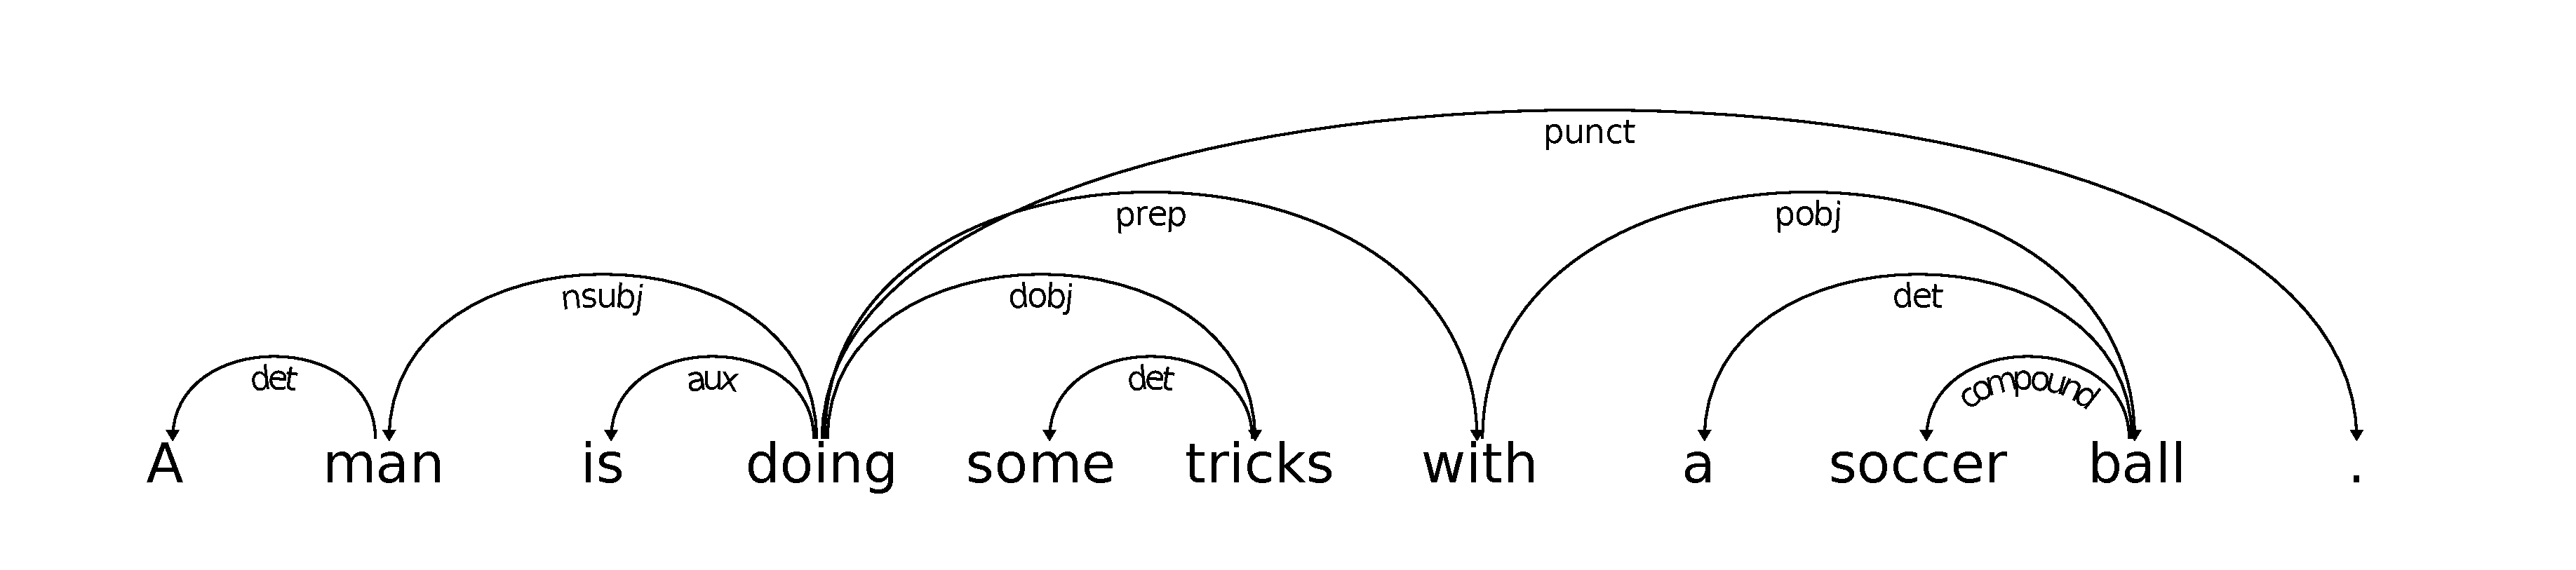
\includegraphics[width=1.\linewidth]{background/depparse_displacy.pdf}
  \caption{Dependency parse tree with typed relations. Arcs point from heads to their dependents. They are labeled with dependency types.}
  \label{fig:displacy_deps}
 \end{figure}


\subsubsection{Dependency Types} \label{subsec:dependency_types}
%Dependents modify their head, but a head governs its dependents. 
 %, similar to a linguistic constituent. 
In addition to structural information given by the dependence relation, dependency grammars classify the kinds of dependencies in terms of the grammatical role the dependent plays with respect to its head. For instance, \textit{subject}, \textit{direct object} or \textit{indirect object} are commonly used and relate to the main finite verb. Because they link phrases of clauses, they are called \textit{clausal argument relations}. To classify all types of dependencies found in dependence structures, the \ac{DG} formalism expands the set of grammatical roles further to types of \textit{nominal modifier relations}, \textit{conjunctions} and many others. Languages vary in the set of dependency types and the means of expressing them (e.g. morphological marker, word order, function words). Nevertheless, efforts are underway to standardize the landscape of considered types of dependency relations. One approach that recently gained attention is the Universal Dependencies project \autocite{nivre_universal_2016}. It defines a common core of 40 grammatical relations while being flexible enough to incorporate language specific types, if needed. The project currently provides resources annotated with dependency structure (treebanks) for 60 different languages.

The English language is comparably restricted in its word order and has weak morphology. As \textcite{jurafsky_dependency_2014} states, in this case, the dependency type strongly correlates with the position of the individual words.

%\todo{UL: How to determine dependency structures? (X)}

\subsubsection{Dependency Parsing} \label{subsubsec:dependency_parsing}
Dependency parsing describes the process of constructing typed dependency structures for a given textual input. This can be done automatically by programs called dependency parsers.

State of the art systems achieve labeled attachment scores (LAS) and labeling scores (LS) of 89.0\% / 93.3\% \autocite{honnibal_improved_2015}\footnote{This parser is part of the spaCy (\url{https://spacy.io/}) \ac{NLP} framework.} or 90.7\% / 94.7\% \autocite{choi_it_2015} at the English OntoNotes corpus \autocite{weischedel_ontonotes_2011}. The authors of the corpus name an inter-annotator agreement of 98.5\% F1 for syntactical annotations on a sampled subset.

%inter-annotator agreement on Stanford Depedencies corpus 96\% for 1,025 tokens \autocite{silveira_gold_2014}



\begin{comment}
\subsection{Transfer Learning}
Successful supervised deep learning depends on access to certain amounts of quality labeled training data. Despite big datasets for some tasks exist by now, that is not every time the case since dataset creation is expensive. However, a lot of tasks and domains share common subsets. Transfer learning aims to exploit these interdependencies by conveying knowledge learned at one domain and task to another. 

Following the notation of \textcite{pan_survey_2010} we define a \textit{domain} $\mathcal{D}$ as $\mathcal{D} = (\mathcal{X}, P(X))$ and a \textit{task} $\mathcal{T}$ as $\mathcal{T} = (\mathcal{Y}, P(Y|X))$ where $\mathcal{X}$ and $\mathcal{Y}$ are feature and label spaces, respectively, $P(X)$ is a marginal probability distribution with $X = \{x_1, ..., x_n\} \in \mathcal{X}$ and $P(Y|X)$ is a conditional probability distribution with $Y = \{y_1, ..., y_m\} \in \mathcal{Y}$\todo{merge notation with previous one}.
Hence, given source and target domains $\mathcal{D}_S$ and $\mathcal{D}_T$ and source and target tasks $\mathcal{T}_S$ and $\mathcal{T}_T$, one can enumerate different qualities of transfer learning:% scenarios/features/qualities(?):
\begin{enumerate}
\item $\mathcal{D}_S \neq \mathcal{D}_T$
\item $P(X_S) \neq P(X_T)$
\item $\mathcal{T}_S \neq \mathcal{T}_T$
\item $P(Y_S|X_S) \neq P(Y_T|X_T)$
\end{enumerate}
where, theoretically, any combination is possible, but usually $(1.) \Rightarrow (2.)$ and $(3.) \Rightarrow (4.)$. 

Training and usage of term embeddings is an instance of transfer learning where conditions $(3.)$ and $(4.)$, and optionally $(2.)$, hold, that is known as unsupervised \textit{feature representation learning}. These and similar approaches in the context of deep learning \autocite{glorot_domain_2011,chen_marginalized_2012}, in fact, implement an \textit{autoencoder} \autocite{bengio_deep_2012}. An autoencoder compresses its input into a small feature vector and tries to reconstruct it from this representation.

\textit{Transductive transfer learning} or \textit{domain adaption} is a scenario where $\mathcal{T}_S = \mathcal{T}_T$, but $P(X_S) \neq P(X_T)$. Taking efficient term embeddings for granted, this work focuses on domain adaption as we examine the effect of pre-training the model on a large corpus based on the PPDB dataset which is further fine-tuned and evaluated on the pertinent domain, the SICK dataset, respectively. 

%domain independence \\
%mixing vs. pre-training/fine-tuning\\
%contrast with multi-task learning \\ 

\end{comment}

\fi
%\newpage
%\section{Related work}

%\subsection{Composition models}
survey \autocite{wang_comparison_2017}; \\
survey on bi-gram composition (psych. ling. mot.) \autocite{mitchell_composition_2010} (e.g. semantic priming); \\
survey on bi-gram comp (sum, mul, RecNN) \autocite{blacoe_comparison_2012} (avg better)
German compounds (bi-gram) \autocite{dima_reverse-engineering_2015}; \\
Skip-thought \autocite{kiros_skip-thought_2015}; \\
RecRNN w/ parse structure \autocite{socher_dynamic_2011,socher_semantic_2012,socher_recursive_2013,tai_improved_2015,wieting_paraphrase_2015}; \\ 
RecRNN (deep) \autocite{irsoy_deep_2014}; \\ 
RecRNN w/o predefined structure \autocite{zhao_self-adaptive_2015,chen_sentence_2015}; \\
doc2vec \autocite{le_distributed_2014,lau_empirical_2016}; \\ 
CNN on bag of words \autocite{kalchbrenner_convolutional_2014}; \\
CNN \autocite{kim_convolutional_2014,hu_convolutional_2014,yin_convolutional_2015,he_multi-perspective_2015}; \\
bi-LSTM + char-embeddings \autocite{ling_finding_2015}; \\
multi-LSTM \autocite{liu_multi-timescale_2015}; \\
deep avg (DAN) \autocite{iyyer_deep_2015}; \\
feature-weighted avg (FCT) \autocite{yu_learning_2015}; \\
functional composition (ling motivated) \autocite{baroni_frege_2014,paperno_practical_2014}; \\
intra- vs extra-sentential context (ling motivated) \autocite{polajnar_exploration_2015}; \\
para + doc embeddings (fixed hierarchical LSTM, auto-encoder)
\autocite{li_hierarchical_2015}; \\  
multilingual \autocite{hermann_multilingual_2014}; \\

AVG vs LSTM on paraphrase \autocite{wieting_towards_2015}
impact of word order \autocite{pham_sentence_2013}

%\subsection{Similarity prediction}
traditional approaches; \\
SemEval-2016 Task 1: STS \autocite{agirre_semeval-2016_2016}; \\
SemEval-2017 Task 1: STS \autocite{cer_semeval-2017_2017}; \\

siamese RNN + manhatten (simple) \autocite{mueller_siamese_2016}; \\

\autocite{habernal_exploiting_2015};
\autocite{boltuzic_identifying_2015};
\autocite{misra_measuring_2016};

%see \autocite{wieting_towards_2015}



%\newpage
%\section{Model architecture and training}
This chapter describes the architecture of the neural model used to calculate a similarity score for a given sentence tuple and how this model is trained.

\subsection{Model architecture}
The model consists of an embedding unit and a similarity function. The embedding unit translates a sequence of tokens into a single embedding vector and is applied to the two input sentences. It calculates the sentence embedding by gathering the individual embeddings for the contained tokens, eventually enhancing them with additional information, and applying a composition function. The two resulting embeddings are fed into the similarity function that produces the similarity score. 

Figure~\todo{AB: add figure} shows this architecture. In the following, we describe the respective modules. 

\subsubsection{Token Embeddings}
We use 300 dimensional GloVe embeddings \todo{AB:explain why} \autocite{pennington_glove_2014} to embed individual word tokens. To evaluate the influence of dependency types, we concatenate the embedding with the one-hot encoded dependency type. The dependency type tag set is based on the Universal Dependencies project \autocite{nivre_universal_2016} and includes 40 different types, resulting in 340 dimensional vectors as input for the composition function. When disabling this feature, we set these 40 entries to zero. The embedding weights are not optimized during training.   

\subsubsection{Composition function}
In this work, we compare two different settings: Using (1) \acf{AVG} or (2) \acf{LSTM} as composition function. 
In the \ac{AVG} case, we apply one \acf{FC} with $tanh$ as activation function to every token embedding. Then, averaging the resulting vectors gives the sentence embedding.
In the \ac{LSTM} setting, the token embeddings are fed directly into a LSTM layer whose output is used as sentence embedding. The two settings are visualized in Figure~\todo{AB: add figure}.

To achieve comparability between the two composition functions, we control the amount of effectively trainable parameters in each of them. Depending on whether dependency parse information is used, we use different sizes for the $tanh$ \ac{FC} in the \ac{AVG} case and the inner state of the \ac{LSTM} to fix the amount of effective parameters to approximately 111000. Table~\ref{tab:sizes} shows the exact amounts and sizes of the elements. % total sizes: AVG=input*fc, LSTM=(input+state+1)*4*state 

\begin{table}[!htb]
  \centering
  \begin{tabular}{ l | c | c }
      & AVG (FC size) & LSTM (state size) \\ \hline
    w/ dependency edge & 110840 (326) & 111248 (68) \\ 
    w/o dependency edge & 111000 (370) & 111000 (74) \\
  \end{tabular}
  \caption{Amounts of trainable parameters and sizes of composition function elements}
  \label{tab:sizes}
\end{table}

\subsubsection{Similarity calculation}
We use the cosine similarity to calculate the similarity score between the two sentence embeddings as described in section~\ref{subsec:similarity_measure}:
\begin{equation}
f_{SIM_{cos}}(a,b) = \frac{a \cdot b}{\norm{a}_2\norm{b}_2} 
\end{equation}

\subsubsection{Baseline model}
As baseline of comparison we calculated TF-IDF based similarity scores in the following manner. We parse and lemmatize each sentence and filter for verbs, nouns and adjectives according to POS tags. Then, we embed each sentence with TF-IDF as described in section~\ref{subsec:doc_embedding} and apply the similarity measure as usual. 

\subsection{Training and Implementation}
We train the model via batched back-propagation with the \ac{MSE} loss function described in section~\ref{subsec:cost_function} and apply ADAM \autocite{kingma_adam_2014} %ADADELTA \autocite{zeiler_adadelta_2012}
as optimizer. We use a 4:1 train/dev split for early stopping. The training is terminated when the score on the development data set does not increase anymore regarding a smoothing window covering the last 25 epochs. 

The model is implemented with the TensorFlow framework  \autocite{abadi_tensorflow_2016}. TensorFlow allows to define and to execute arbitrary dataflow graphs efficiently on different devices as CPUs or GPUs. For tokenization and dependency parsing we use spaCy\footnote{see \url{https://spacy.io/}} which is a fast and still accurate\footnote{see \textcite{choi_it_2015} for a comparative study} \ac{NLP} framework. 


%\subsection{Pre-Training}
%To increase the amount of available training examples, we examined pre-training on a dataset that is one order of magnitude larger than the SICK corpus. We train the models on this data until the early stopping criterion is met and use the resulting weights to initialize the models trained on the SICK dataset. 





%\newpage
%\section{Experiments and Evaluation}

\subsection{Datasets}

\subsubsection{BioASQ}
train + evaluate; Pubmed-abstract -> Mesh terms; multiclass prediction; ca. 10k classes; use only structured abstracts -> ca. 4m docs
\todo{AB: distribution of text lengths?}

\subsubsection{DBpedia-NIF}
pre-train (+ evaluate); two Wikipedia articles -> relatedness score; similarity prediction; ca. 5m docs
\todo{AB: distribution of text lengths?}

\subsection{Training and Hyperparameters}
batched gradient descent; max entropy loss; adam optimizer; gradient clipping; dropout; \\
train word embeddings for words not in initial (glove + biomedical) embeddings \\
for relatedness prediction: negative sampling 

\subsection{Results}
total (no pre-training; min 170 occurrences per word type/MeSH tag!; F1-scores): \\
tf-idf: 0.64  > RecNN: 0.63 > flat(sum): 0.60 > RNN: 0.50 \\
different results for different text sizes? -> train \& evaluate on text-size-buckets

\if false
===OLD SRP CONTENT===

We conduct several experiments to evaluate the influence of order awareness and availability of dependency type information to the similarity prediction performance. We test all combinations of the boolean parameters \texttt{dependency available} and \texttt{order aware} and the TF-IDF baseline. In the following, we describe the dataset and the hyperparameter setting. Finally, we present the results including a comparative analysis of errors.

\subsection{Dataset}
We use the SICK corpus\footnote{\url{http://alt.qcri.org/semeval2014/task1/index.php?id=data-and-tools}} \autocite{marelli_sick_2014} for model training and evaluation. The corpus consists of about approximately 10.000 pairs of English sentences based on the 8K ImageFlickr data set\footnote{\url{http://nlp.cs.illinois.edu/
HockenmaierGroup/data.html}} \autocite{hodosh_framing_2013} and the SemEval 2012 STS MSR-Video Description data set\footnote{\url{https://www.cs.york.ac.uk/semeval-2012/task6/index.php\%3Fid=data.html}} \autocite{agirre_semeval-2012_2012} that contain sentences describing the same picture or video. These sentences were linguistically normalized; i.e. Named Entities and complex verb constructions are replaced and subordinates are turned into coordinates. Pairs were manually %expanded to generate candidate pairs that were 
labeled by 10 annotators with one to five point relatedness ratings that are averaged to produce a relatedness score. We rescaled the scores into the interval $[0.0, 1.0]$ to let them fit into our definition of a similarity measure. Table~\ref{tab:sick_examples} shows some examples of the dataset. The mean of the score for both train and test set is approximately $0.63$. The sentences contain $2408$ different token types and have an average length of $9.6$ words.  

We chose the SICK corpus because it was used in the SemEval 2014 task 1\footnote{\url{http://alt.qcri.org/semeval2014/task1/}}, thus it is widely studied and various reference systems exist. Furthermore, as stated by \textcite{marelli_semeval-2014_2014}, this corpus was created to evaluate semantical aware composition without relying on too many external tools and resources (e.g., named-entity recognizers, gazetteers, ontologies).
%mean score: 0.63 * 4.0 + 1.0 = 3.53

\begin{table*}[!htb]
\centering
  \begin{tabular}{p{0.4\textwidth}|p{0.4\textwidth}|c}
    sentence A & sentence B & score \\ \hline \hline
    A man in a shirt dyed purple is looking at a man in a black shirt who is doing a funny face & A man in a shirt dyed purple is looking at a man in a black shirt who is doing a face which looks funny & 1.0 \\ \hline
    A group of kids is playing in a yard and an old man is standing in the background & A group of boys in a yard is playing and a man is standing in the background & 0.875 \\ \hline
    A brown dog is attacking another animal in front of the man in pants & Two dogs are wrestling and hugging & 0.55 \\ \hline
    A woman is chopping an onion & A woman is washing her feet & 0.0
  \end{tabular}
  \caption{Example sentence pairs from SICK corpus with rescaled relatedness score ranging from $0.0$ (not related) to $1.0$ (maximal related).}
\label{tab:sick_examples}
\end{table*}

%\subsubsection{SICK}

%\subsubsection{PPDB}
%Our pre-training dataset is based on the phrasal part of the PPDB 2.0 dataset \autocite{pavlick_ppdb_2015}. We use a subset of 100,000 paraphrases and add an equal amount of negative samples by replacing for each pair the second paraphrase entry with a random phrase sampled uniformly\footnote{We also tried to sample according to the Jaccard similarity distribution of the original pairs, but this decreased the performance.} from all existing second pair entries. A similarity score of 1.0 is assigned to the original paraphrase pairs, the negative samples are scored with 0.0.

\subsection{Training and Hyperparameters}
We train the model in batches of 100 examples. The ADAM optimizer is initialized with a learning rate of 0.003. We apply gradient clipping by global norm as specified in \textcite{pascanu_difficulty_2012} with a threshold of 5.0 and use dropout \autocite{srivastava_dropout_2014} with a keep probability of 0.8 at the \ac{LSTM} and the \ac{FC} in the \ac{AVG} case to prevent from overfitting. We used a grid search at the train/dev set to find this parameter configuration. We applied 5-fold cross validation with regard to the train/dev split for every setting and repeated each experiment 10 times to achieve robust results.

\subsection{Results}
We measured performance using the Pearson correlation coefficient and \ac{MSE} between the predictions and gold scores. The mean Pearson correlation of all 200 runs\footnote{4 settings $\times$ 5-fold cross validation $\times$ 10 repetitions} is about $0.839$ %\todo{UL: Wie weit vom Inter-Annotator-Agreement? Lohnen sich weitere Verbesserungen? (X)} 
with a \ac{STD} of $0.002$ and the mean \ac{MSE} is $0.024$ with \ac{STD} of $0.004$. The \ac{TF-IDF} baseline produces a Pearson score of $0.619$ and a \ac{MSE} of $0.082$. Thus, the regarded models achieve a mean \ac{MSE} performance gain of $+6.4$ pph (parts per hundred) with respect to the baseline. Note, that the authors of the SICK corpus name an inter-annotator agreement of 0.036 in means of variance.\footnote{Precisely, the authors present a standard deviation of 0.76. Rescaling from the original scoring range $[1, 5]$ into the range $[0, 1]$ used in this work leads to the mentioned variance value.} 

The performance of the Order Aware model (MSE: $0.0206$; Pearson's~r: $0.838$) lies in the range of the best system submitted for SemEval-2014 relatedness prediction task (MSE: $0.020$, Pearson's~r: $0.828$), but stays below state of the art. Recent systems achieve MSE/Pearson's~r scores of $0.016$/$0.87$ \autocite{he_multi-perspective_2015}(CNN) or $0.014$/$0.88$ \autocite{mueller_siamese_2016}(LSTM) without exploiting dependency information (Section~\ref{sec:related_work}). We list the individual performances of the models examined in this work averaged over identical parameter settings in Table~\ref{tab:results}. Figure~\ref{fig:res_all} displays the \ac{MSE} and Pearson's~r results for all parameter combinations as box plots\footnote{The boxes of all box plots show the \ac{IQR}, whiskers mark the $[1.5\times \text{IQR}, 3\times \text{IQR}]$ range and notches the  $10000\times$ bootstrapped confidence intervals.}. Note, that the y-axis is inverted for all box plots visualizing \ac{MSE} scores to show better performing scores above worse ones and to provide comparability with plots of Pearson scores. 
%# SICK_VERBADJNOUN_lemma	0.611	0.091		# TFIDF
%# SICK_ADJNOUN_lemma	0.558	0.111			# TFIDF
%# SICK_VERBADJNOUN_orth	0.568	0.106		# TFIDF
%# SICK_ADJNOUN_orth	0.542	0.119			# TFIDF

%\begin{figure}[htb!]
%  \centering
%  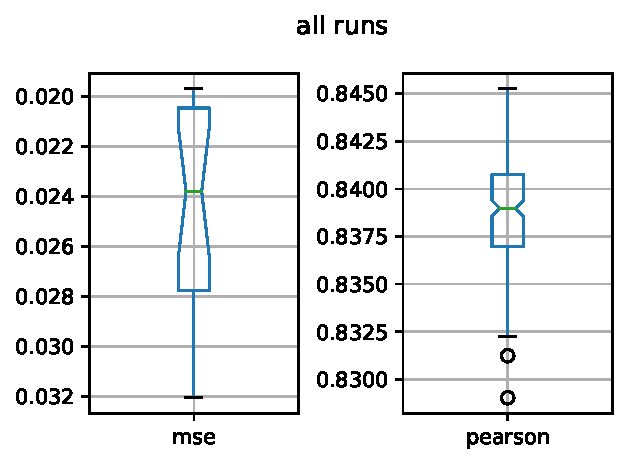
\includegraphics[width=0.9\textwidth]{results/fig_merged.pdf}
%  \caption{Overall model performance as Pearson correlation and MSE.}
%  \label{fig:res_merged}
%\end{figure}

%\begin{figure}[htb!]
%  \centering
%  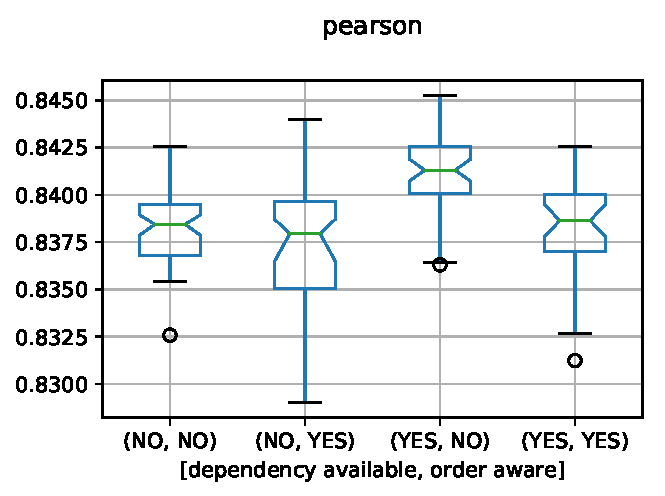
\includegraphics[width=0.9\textwidth]{results/fig_sep_pearson.pdf}
%  \caption{Pearson correlation scores for the different settings.}
%  \label{fig:res_sep_pearson}
%\end{figure}

%\begin{subtable}[c]{\textwidth}
%	\centering
\begin{table}[htb!]
  	\centering
  	%\begin{tabular}{|l|l|l|}
 \begin{tabularx}{
 		\textwidth}{|p{0.26\textwidth} p{0.25\textwidth}|X|X|}%{|X X|X|X|}
 %\begin{tabularx}{\textwidth}{|p{0.21\textwidth} p{0.15\textwidth}|X|X|} %{p{0.4\textwidth}|p{0.4\textwidth}|c}
		\hline
		\texttt{dependency available} & \texttt{order aware} & mse & pearson \\ \hline \hline
		NO & NO & 0.0284 & 0.8382 \\ 
		NO & YES & 0.0206 & 0.8375 \\
		YES & NO & 0.0274 & 0.8413 \\
		YES & YES & 0.0205 & 0.8383 \\ \hline \hline
		\multicolumn{2}{|l|}{TFIDF} & 0.0823 & 0.6189 \\ \hline
 \end{tabularx}
 %\captionsetup{width=0.9\linewidth}
 \caption{MSE and Pearson scores aggregated by setting.}
 \label{tab:results}
\end{table}
%	\vspace*{0.8 cm} \newline
	
  %\caption{Average \ac{MSE} and Pearson's r scores}
%\end{table}


\begin{figure}[htb!]
  \centering
  \textbf{Overall performance by setting}\par\medskip
  \begin{subfigure}{.5\textwidth}
    \centering
    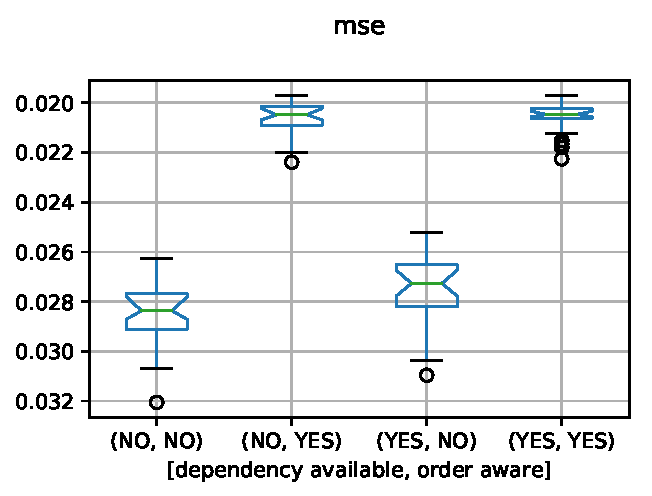
\includegraphics[width=1.\linewidth]{results/fig_sep_mse.pdf}
    \captionsetup{width=0.9\linewidth}
    %\caption{MSE for the different settings (inverted y-axis).}
  \end{subfigure}%
  \begin{subfigure}{.5\textwidth}
    \centering
    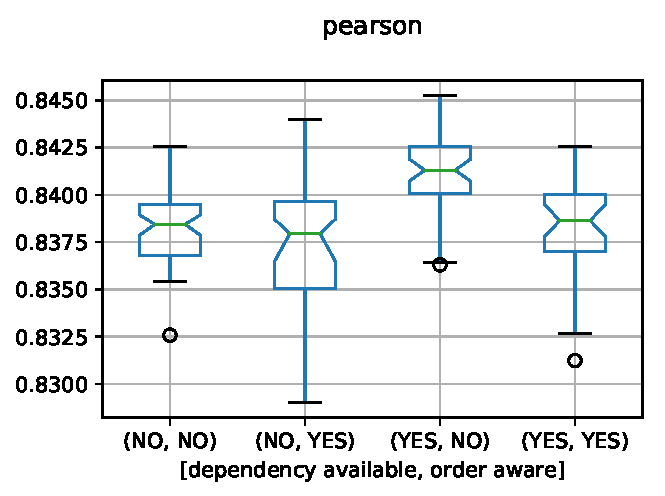
\includegraphics[width=1.\linewidth]{results/fig_sep_pearson.pdf}
    \captionsetup{width=0.9\linewidth}
    %\caption{Pearson's r for the different settings.}
  \end{subfigure}
  \caption{MSE (inverted y-axis) and Pearson's r for the different settings.}
  \label{fig:res_all}
\end{figure}

Adding \textbf{dependency types} improves on average \ac{MSE} by $0.05\%$ and Pearson's r increases by $0.24$ pph, whereby the former is not significant (p=0.336), but the later is ($p<0.0001$). Enabling the feature \textbf{order aware} results in a significant overall performance gain of $0.75$ pph  in means of \ac{MSE} and a performance decrease of $-0.21$ pph with regard to Pearson's r ($p<0.0001$ for two-tailed t-test in both cases). Table~\ref{tab:results_merged} shows the specific scores.

\begin{table}[htb!]
	\centering
	\begin{tabularx}{\textwidth}{|p{0.22\textwidth} p{0.13\textwidth}|p{0.11\textwidth} X|p{0.11\textwidth} X|} 
		%\begin{tabularx}{\textwidth}{|p{0.21\textwidth} X|X|X|} %{p{0.4\textwidth}|p{0.4\textwidth}|c}
		\hline
		parameter & enabled & mse & & pearson  & \\ \hline \hline
		dependency type & NO & 0.0245 & & 0.8378 & \\
		dependency type & YES & 0.0240 & $+0.05$ pph* & 0.8398 & $+0.24$ pph \\ \hline
		order aware & NO & 0.0279 &  & 0.8397 &  \\
		order aware & YES & 0.0206 & $+0.75$ pph & 0.8379 & $-0.21$ pph \\ \hline	   		
	\end{tabularx}
	%\captionsetup{width=0.9\linewidth}
	\caption{Scores aggregated by individual parameter assignment and improvement when enabling the feature. The improvement marked with (*) is not significant.}
	\label{tab:results_merged}
\end{table}

For further study these results that seem to contradict with respect to the applied measure, we took a closer look at the deviations of the predicted relatedness scores from the gold scores. Figure~\ref{fig:fig_sorted_errors_sep} shows the deviations per setting ordered by gold score. It suggests that the averaging model (\texttt{order aware} = NO) overestimates the relatedness score. Indeed, the bias for all predictions in the averaging case ($+8.5$ pph) is significantly ($p < 0.0001$) higher when compared with non-averaging ($+1.9$ pph). Because such a bias distorts the Pearson's~r, and \ac{MSE} was used as cost function while training, we focus at the \ac{MSE} measure for the rest of this work.

\begin{figure}[htb!]
	\centering
	\textbf{Deviations from gold score}\par\medskip
	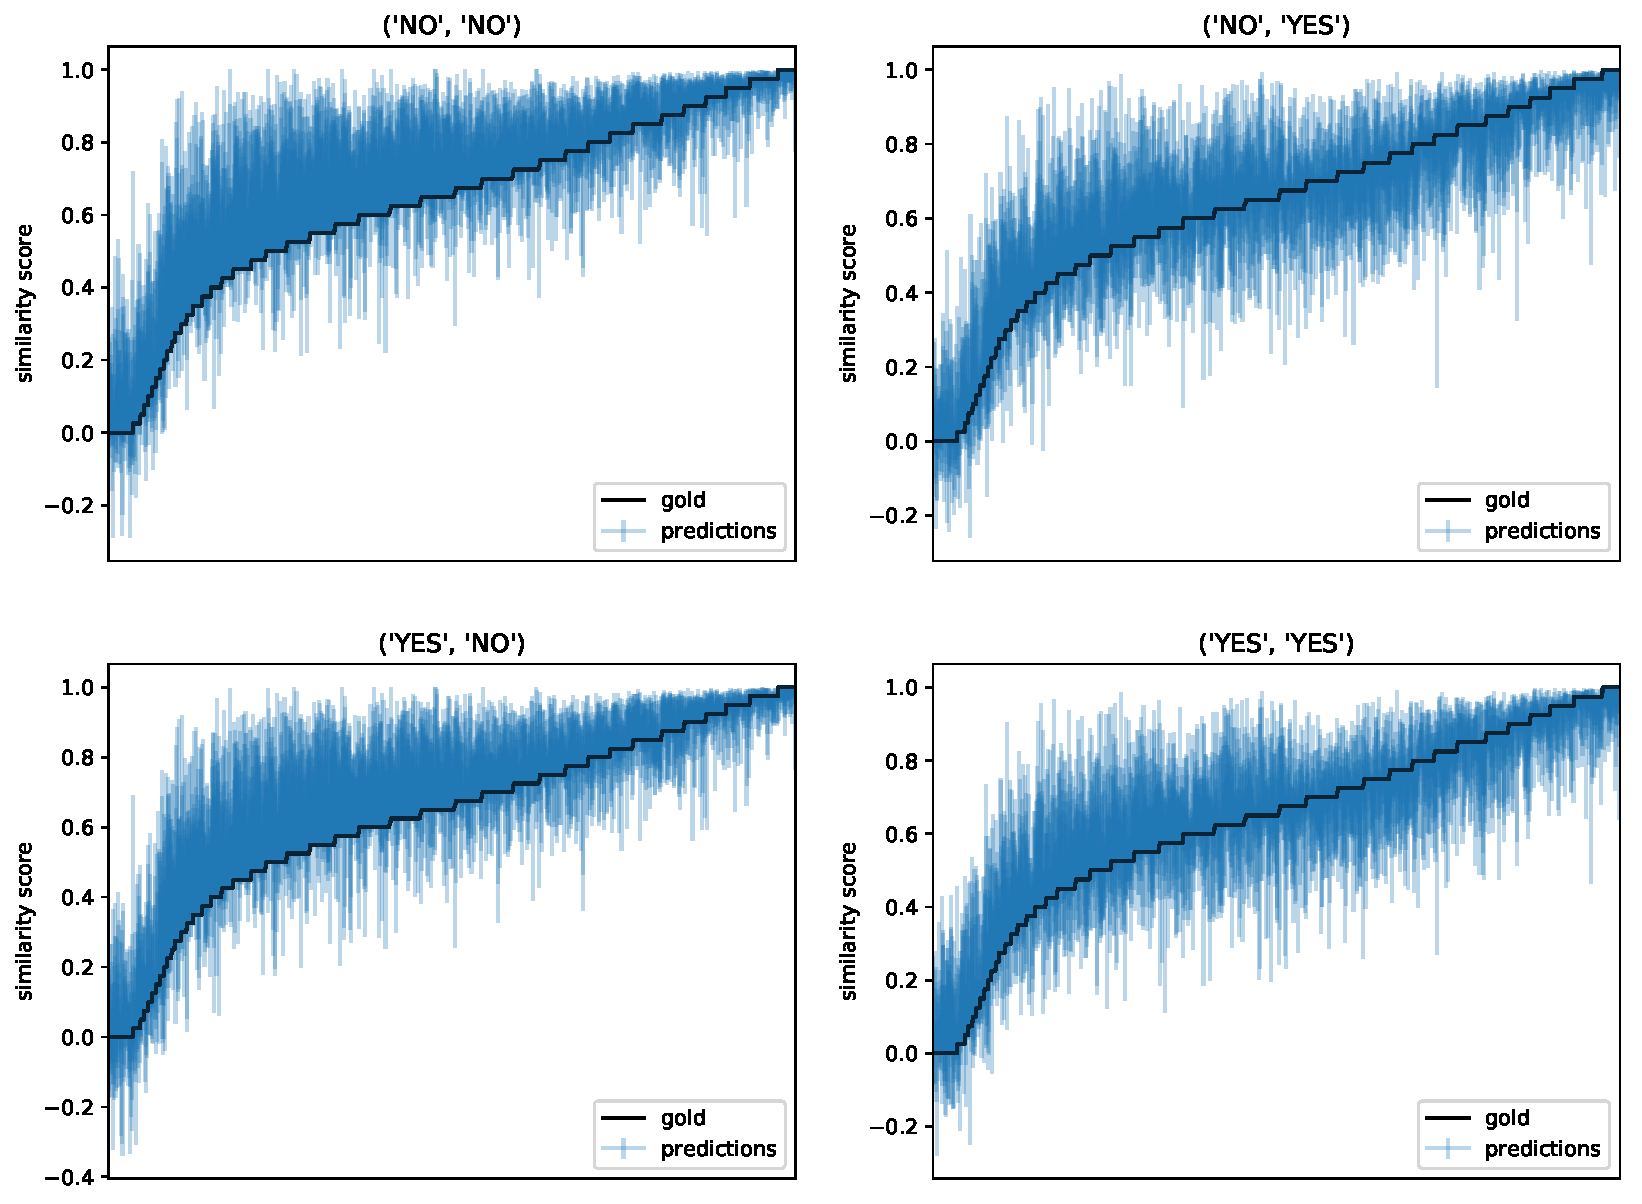
\includegraphics[width=1.\linewidth]{results/fig_sorted_errors_sep.pdf}
	\caption{Deviations of the predictions from gold similarity scores by setting (<\texttt{dependency available}>, <\texttt{order aware}>). The averaging models (\texttt{order aware} = NO; plots at the left) clearly overestimate.}
	\label{fig:fig_sorted_errors_sep}
\end{figure}

\subsubsection{Relation of Order Awareness and Dependency Types} \label{subsec:results_relation_OA_DA}
The specific performance in the examined settings suggests that the parameters \texttt{dependency available} and \texttt{order aware} are related. Figure~\ref{fig:fig_sep_cond} illustrates this by presenting the conditional impact of the parameters. The impact of \texttt{dependency available} seems to vary depending on activation of parameter \texttt{order aware}, whereas the opposite does not hold (see Table~\ref{tab:results} for the actual values). This observation leads to the following question: What kind of useful information with respect to semantical awareness is encoded in dependency types? Precisely, we assume: Dependency types encode local context information that is useful to produce semantic aware compositional representations. The rationale is as follows. 
Order Awareness as implemented within \ac{LSTM}s enable locally contextualized processing (see Section~\ref{subsec:order_aware_composition}). Thus, these models encode local context.
As explained in section \ref{subsec:eval_semantic_awareness}, semantic awareness can be measured using the relatedness prediction task. Since enabling the parameter \texttt{order aware} significantly increases the prediction performance by $+0.8$ pph ($p < 0.0001$) the local context information seems to be important to determine the meaning of a word in a specific textual utterance and to handle semantic aware composition.
Enabling the parameter \texttt{dependency available} significantly improves the model performance by $+0.1$ pph ($p < 0.001$) in the case of disabled order awareness, proving that dependency types indeed encode \textbf{useful} information.
Since the order aware model does not perform significantly better with dependency type data ($t = 0.50$) it seems that this data does not encode extra useful information for order aware models.
This suggests that dependency types indeed encode \textbf{local context}.

\begin{figure}[htb!]
	\centering
	\textbf{Conditional parameter impact}\par\medskip
	\begin{subfigure}{.5\textwidth}
		\centering
		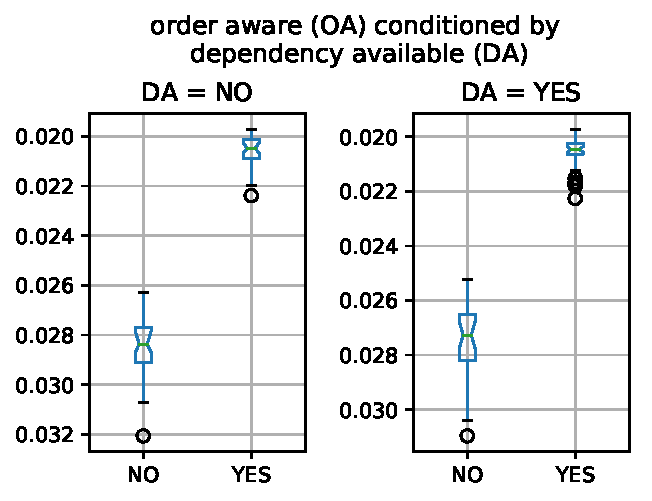
\includegraphics[width=1.\linewidth]{results/fig_sep_cond_order.pdf}
		%\captionsetup{width=0.9\linewidth}
		%\caption{Impact of parameter \textit{order aware} conditioned by enabled \textit{dependency available} parameter.}
	\end{subfigure}%
	\begin{subfigure}{.5\textwidth}
		\centering
		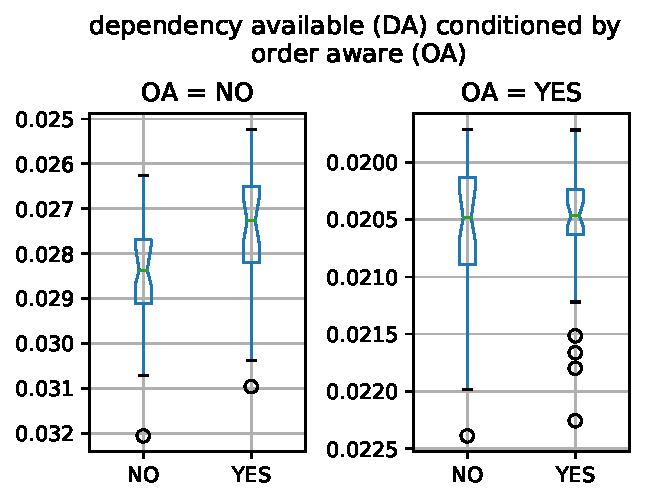
\includegraphics[width=1.\linewidth]{results/fig_sep_cond_dependency.pdf}
		%\captionsetup{width=0.9\linewidth}
		%\caption{Impact of parameter \textit{order aware} conditioned by disabled \textit{dependency available} parameter.}
		\captionsetup{width=0.9\linewidth}
		%\caption{Impact of parameter \textit{dependency available} conditioned by parameter \textit{dependency available}.}
	\end{subfigure}	
	\caption{Conditional parameter impact measured with MSE.}
	\label{fig:fig_sep_cond}
\end{figure}


%\begin{figure}[htb!]
%  \centering
%  \includegraphics[width=0.9\textwidth]{fig_sep_order.pdf}
%  \caption{Influence of order awareness measured with Pearson correlation and MSE.}
%  \label{fig:pearson_all_sep}
%\end{figure}

%\subsubsection{cosine vs. manhattan}
%\subsubsection{Dependency edge types}
%mean mse: 0.0245 -> 0.0240 =  -0.0005 \\
%mean pearson: 0.8378 -> 0.8398 =   0.0019 \\
%performance gain of 0,05\%*/0,31\% (mse/pearson) regarding TF-IDF baseline 

%*: not significant
%\begin{figure}[htb!]
%  \centering
%  \includegraphics[width=0.9\textwidth]{fig_sep_dep.pdf}
%  \caption{Influence of dependency edge type Information measured with Pearson correlation and MSE.}
%  \label{fig:pearson_all_sep}
%\end{figure}



%\subsubsection{Pretraining}

\subsubsection{Value of Dependency Types}
In order to further investigate the value of dependency type data for semantic aware composition we have taken a closer look at the sentence pairs in which only adding this data outperforms the setting in which parameter \texttt{order aware} is enabled exclusively. Table~\ref{tab:results_benefit_DA} lists the top 10 of these data points. Trying to examine the reasons behind cases of superior performance reveals two main classes of constructions (see column \textit{remarks} of Table~\ref{tab:results_benefit_DA}). First, half of the top 10 sentence pairs contains passive constructions. Second, three sentence pairs are related to negation. 

As it turns out, dependency type data seems to be beneficial to handle composition of tokens involved in passive constructions. We filtered the test data set for dependency types indicating these constructions (\textit{auxpass}: passive auxiliary; \textit{nsubjpass}: passive nominal subject; \textit{csubjpass}: passive clausal subject) and calculated \ac{MSE} scores\footnote{We used the relatedness scores predicted by the best model for each setting with respect to train/test split and run.}. Table~\ref{tab:mse_passive} presents the resulting scores and subset sizes. Figure~\ref{fig:fig_mse_passive} visualizes the results. The Dependency Available setting ([YES, NO]) significantly ($p < 0.0001$) outperforms the Order Aware setting ([NO, YES]) in the presence of passive constructions. Furthermore, negation seems to be hard in general. Similar to the passive check, we selected a subset of the test dataset, but filtered by dependency type \textit{neg} and words like "no" or "nobody". For all four settings, the performance dropped significantly when switching from the subset without negation to the negation subset. Despite initial thoughts, negation favors Order Awareness (e.g., performance drop of $-0.2$ pph for [NO, YES] vs. $-0.5$ pph for [YES, NO]) as visualized in Figure~\ref{fig:fig_mse_negation}. Again, Table~\ref{tab:mse_passive} displays the specific evaluation scores and, in addition, relative performance differences with respect to the considered data split.

% pearson-correlation("('NO', 'NO') vs ('YES', 'NO') abs"; "score_jaccard") = -0.456
% > increasing overlap -> decreasing benefit of "dependency available" 
Obviously, the benefit of dependency types decreases with increasing word overlap. Correlating the absolute differences of prediction errors of settings [NO, NO] and [YES, NO] with the Jaccard similarity $f_{S_\text{Jacc}}$\footnote{$f_{S_\text{Jacc}}(s_1, s_2) := \frac{\text{\#(set of tokens in $s_1$ \texttt{AND} $s_2$)}}{\text{\#(set of tokens in $s_1$ \texttt{OR} $s_2$)}}$} of the respective sentences results in a Pearson's r of $-0.46$ indicating a moderate negative correlation.

\begin{table}[htb!]
	\centering
	\begin{tabularx}{\textwidth}{p{0.35\textwidth}|p{0.35\textwidth}|X|X} 
		%\begin{tabularx}{\textwidth}{|p{0.21\textwidth} X|X|X|} %{p{0.4\textwidth}|p{0.4\textwidth}|c}
		\hline
		sentence A & sentence B & errors & remarks \\ \hline \hline
		The patient is being helped by the doctor & The doctor is helping the patient & $-.0;-.5$ (1.0) & passive \\ \hline
		The panda bear is not lying on the logs & A cute panda is lying down & $-.2;-.7$ (0.8) & negation \\ \hline
		A man and a woman are sitting comfortably on the bench & Two large persons are sitting on a park bench and they have a bottle of soda between them & $-.1;-.5$ (0.7) & appended "noise" \\ \hline
		A man is not playing a guitar & A man is playing a keyboard & $-.1;-.4$ (0.7) & negation \\ \hline
		A dog is standing with its two front paws on a rock in a field & A rock is being climbed by the black dog & $-.1;-.4$ (0.6) & passive \\ \hline
		Four middle eastern children, three girls and one boy, are climbing on the grotto with a pink interior & The grotto with a pink interior is being climbed by four middle eastern children, three girls and one boy & $-.0;-.3$ (1.0) & passive \\ \hline
		The flute is being played by one man & A man is playing the guitar loudly & $-.0;-.3$ (0.6) & passive \\ \hline
		Nobody is dangling from straps and kicking at each other & A blonde girl is hanging by gymnastic ropes & $-.1;-.4$ (0.4) & negation \\ \hline
		A child is making a snow ball & A snow ball is being made by a child & $-.0;-.3$ (1.0) & passive \\ \hline
		A black cat and a small white and black cat are looking up at a kitchen countertop & A large dog and a small dog are standing next to the kitchen counter and are investigating & $-.0;-.3$ (0.4) &  \\
		\hline \hline	
	\end{tabularx}
	%\captionsetup{width=0.9\linewidth}
	\caption{The top 10 sentence pairs where enabling \texttt{dependency available} (setting: [YES, NO]) outperforms enabling \texttt{order aware} (setting: [NO, YES]). Rounded deviations from gold scores for both settings ([YES, NO]; [NO, YES]) are presented as \textit{errors} with the actual gold score (rounded) in brackets. The \textit{remarks} column names sources of potentially beneficial effects in favor of the Dependency Available setting.}
	\label{tab:results_benefit_DA}
\end{table}


\begin{table}[htb!]
	\centering
	\begin{tabularx}{\textwidth}{p{0.15\textwidth}|XX|XX|XX|XX|p{0.07\textwidth}} 
		 test data & \multicolumn{2}{c}{[NO, NO]} & \multicolumn{2}{|c|}{[NO, YES]} & \multicolumn{2}{c}{[YES, NO]} & \multicolumn{2}{|c|}{[YES, YES]} & count \\ \hline
		 all & 0.028 & & 0.020 & & 0.026 & & 0.020 & & 4927 \\ \hline
		 w/o passive & 0.028 & & 0.019 & & 0.027 & & 0.020 & & 4371 \\
		 w/ passive & 0.023 & $+0.5\%$ & 0.022 & $-0.3\%$ & 0.021 & $+0.6\%$ & 0.021 & $-0.1\%$ & 556 \\ \hline
		 w/o negation & 0.026 & & 0.019 & & 0.025 & & 0.019 & & 3856 \\
		 w/ negation & 0.032 & $-0.6\%$ & 0.021 & $-0.2\%$ & 0.030 & $-0.5\%$ & 0.021 & $-0.2\%$ & 1071 \\
	\end{tabularx}
	%\captionsetup{width=0.9\linewidth}
	\caption{\ac{MSE} for selected subsets of SICK test data measured within all settings ([<\texttt{dependency available}>, <\texttt{order aware}>]) and relative performance gains/drops (+/-) in pph (\%). \textit{count} represents the number of sentence pairs in the respective subset.}
	\label{tab:mse_passive}
\end{table}

\begin{figure}[htb!]
	\centering
	%\textbf{MSE for specific test data subsets}\par\medskip
	%\caption{MSE for specific test data subsets}
	\textbf{Impact of Order Awareness and Dependency Information \\ in the presence of Passive and Negation}\par\medskip
	\begin{subfigure}[t]{.5\textwidth}
		%\centering
		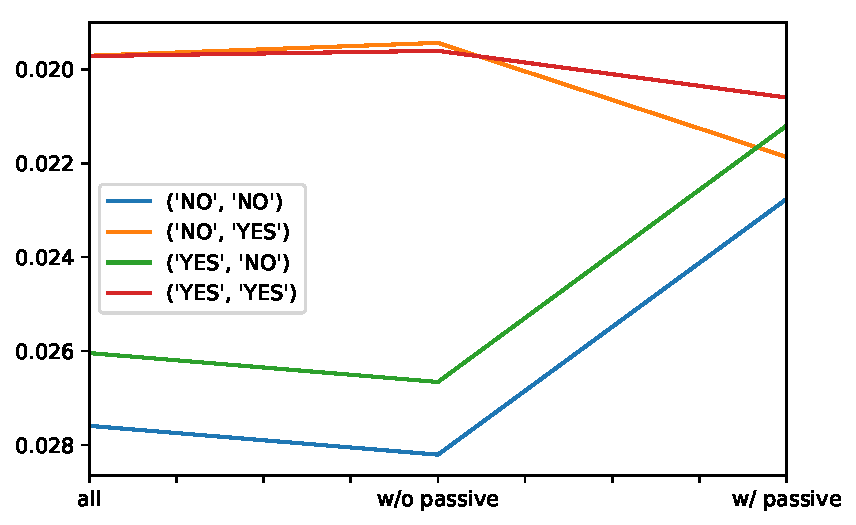
\includegraphics[width=1.\linewidth]{results/fig_mse_passive.pdf}
		\captionsetup{width=0.9\linewidth}
		\caption{The Dependency Available setting ([YES, NO]) outperforms the Order Aware setting ([NO, YES]) on passive constructions.}
		\label{fig:fig_mse_passive}
	\end{subfigure}%
	\begin{subfigure}[t]{.5\textwidth}
		%\centering
		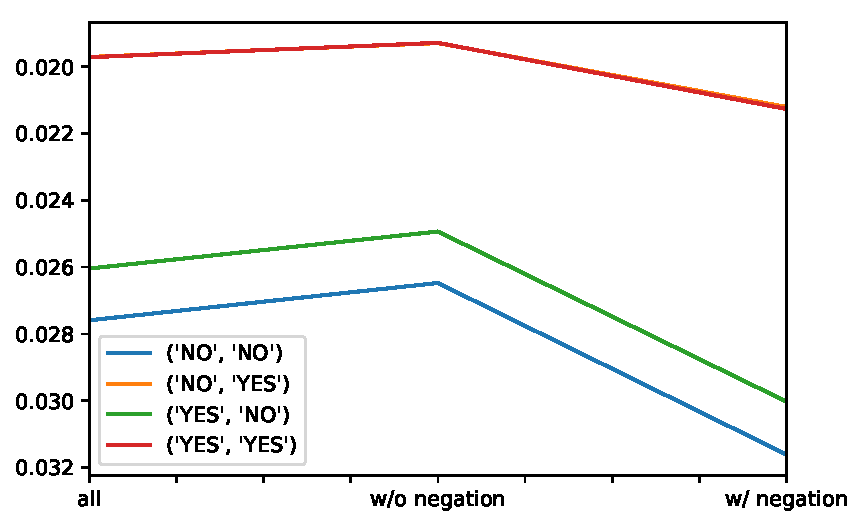
\includegraphics[width=1.\linewidth]{results/fig_mse_negation.pdf}
		\captionsetup{width=0.9\linewidth}
		\caption{The performance decreases for all settings in the presence of negation, but favors Order Awareness ([NO, YES] and [YES, YES]).}
		\label{fig:fig_mse_negation}
	\end{subfigure}	
	\caption{MSE for specific test data subsets}
	%\caption{Conditional parameter impact measured with MSE.}
	%\label{fig:fig_sep_cond}
\end{figure}


\fi

%\newpage
%\clearpage
%\section{Discussion and Future Work}

In line with \textcite{mueller_siamese_2016,iyyer_deep_2015}, our results demonstrate that simple neural models perform quite well for semantic aware composition. Furthermore, we investigated the relation of dependency type data and order aware composition. In this chapter we discuss our findings.% and conclude... 

As demonstrated in Chapter~\ref{subsec:results_relation_OA_DA} locally contextualized processing of individual tokens does matter. That capability is achieved by order aware \ac{RNN} models holding previously processed information in an internal state which is considered to analyze the next token. By keeping the internal state reasonable in size, bottleneck effects induce localization. It suggests, that this kind of contextualization leverages performance by filtering relevant information similar to processes like word sense disambiguation. But it does not look like sequential processing is a requirement. In addition to several well performing \ac{CNN} models, one might imagine to process every individual token in a bag of words manner, but incorporating a vector representation previously created from this bag of words, or in a n-grams fashion, eventually. This mechanism builds upon \textit{attention} \autocite{bahdanau_neural_2014, vaswani_attention_2017} and is called self-attention or intra-attention \autocite{cheng_long_2016} that seems to perform well on semantic \ac{NLP} exploiting very little% or no\footnote{That is meant with respect to a certain area, e.g. a sentence, defining a context frame by itself. As reasoned above, \textit{any} contextualization is important.} 
ordering information \autocite{parikh_decomposable_2016}.%, but despite of, provides a local context. 
Further experiments taking some of these insights into account could be arranged by simply shuffling the sentence tokens and repeating our experiments. By doing so, the context is artificially enlarged to cover the hole sentence and one might investigate, if \ac{RNN} models still strongly outperform averaging of independently mapped embeddings. Likely this requires to use Bi-LSTMs \autocite{graves_speech_2013} or similar architectures, that provide information regarding all previous and following tokens at every position.

%One might expect, that the \acp{RNN} still outperform averaging as they allow contextualization in a manner that is more expressive, as t% and the impact of . % 

Even though all models examined in this work conceptually have access at comparison level (similarity measure application, see Section~\ref{subsec:architecture}) to all relevant information included in the respective embeddings, intermediate sentence representations functioning as bottleneck prevent that, which underpins the benefit of local filtering. To proof this idea, one could expand our models by adding eventually deep networks on top of the individual sentence embedding layer similar to \textcite{iyyer_deep_2015} and increase the dimension of internal sentence representations. Thus, the performance advantage of the order aware models should decrease.

Furthermore, we argued that locally contextualized processing as exploited by order aware models can be achieved by adding dependency type information. As mentioned in \ref{subsec:dependency_types}, order information strongly correlates with dependency type data for English language. Thus, 


ADD CONTENT

% Alternations / Diathese
%http://ling.uni-konstanz.de/pages/home/hautli/LR/verb-classes-levin.pdf
%http://ccl.pku.edu.cn/973_sem_spec/Sem_ling/English%20Verb%20Classes%20and%20Alternations%20A%20Preliminary%20Investigation.pdf

%context -> word sense disambiguation

% what does contextualized processing mean? when is it necessary?
% 1) needs "memory" (internal state)

% contextualization: related to attention?


% SICK is artificial: pros/cons?


% strange Pearson scores
%\newpage
%\section{Conclusion}
%\section{Method/Model/Theory}\label{Sec:Method}

\begin{itemize}

    \item How was the data analyzed ?

    \item Present the underlying economic model/theory and
        give reasons why it is suitable to answer the given problem.

    \item Present econometric/statistical estimation method and
        give reasons why it is suitable to answer the given problem.

    \item Allows the reader to judge the validity of the study and
        its findings.

    \item Depending on the topic this section can also be split up
        into separate sections.

\end{itemize}

%\newpage
%\section{Data}\label{Sec:Data}

\begin{itemize}

    \item Describe the data and its quality.
    \item How was the data sample selected?
    \item Provide descriptive statistics such as:
        \begin{itemize}
            \item time period,
            \item number of observations, data frequency,
            \item mean, median,
            \item min, max, standard deviation,
            \item skewness, kurtosis, Jarque--Bera statistic,
            \item time series plots, histogram.
        \end{itemize}
    \item For example:
        \begin{table}[ht]

        \begin{center}
            {\footnotesize
            \begin{tabular}{l|cccccccccc}
                \hline \hline
                           & 3m    & 6m    & 1yr   & 2yr   & 3yr   & 5yr   & 7yr   & 10yr  & 12yr  & 15yr   \\
                \hline
                    Mean   & 3.138 & 3.191 & 3.307 & 3.544 & 3.756 & 4.093 & 4.354 & 4.621 & 4.741 & 4.878  \\
                    StD    & 0.915 & 0.919 & 0.935 & 0.910 & 0.876 & 0.825 & 0.803 & 0.776 & 0.768 & 0.762  \\
                \hline \hline
            \end{tabular}}
        \end{center}
        \caption{Some descriptive statistics of location and dispersion for
        2100 observed swap rates for the period from February 15, 1999
        to March 2, 2007. Swap rates measured as 3.12 (instead of 0.0312). See Table
        \ref{Tab:DescripStatsRawDataDetail} in the appendix for
        more details.}
        \label{Tab:DescripStatsRawData}
        \end{table}

    \item Allows the reader to judge whether the sample is biased or to evaluate possible impacts of outliers, for
    example.

\end{itemize}

%\newpage
%\section{Results}\label{Sec:Results}

\begin{itemize}

    \item Organize material and present results.

    \item Use tables, figures (but prefer visual presentation):
        \begin{itemize}
            \item Tables and figures should supplement (and not duplicate) the
                text.

            \item Tables and figures should be provided with
            legends.\\
                {\it Figure \ref{Fig:Resids} shows how to include and reference
                graphics. The graphic must be labelled before. Files must be in
                \texttt{.eps} format.}

                \begin{figure}[ht]
                \begin{center}
                    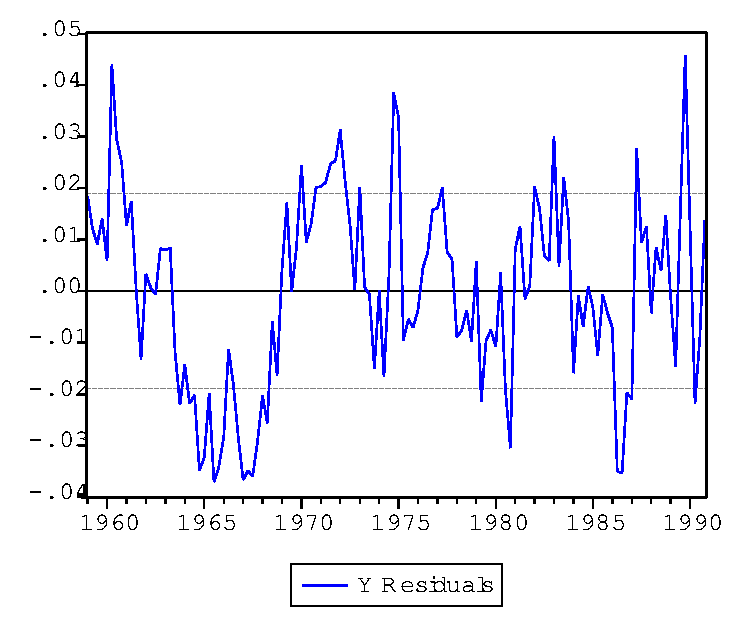
\includegraphics[scale=0.5,angle=0]{graph}
                    \caption{Estimated residuals from model XXX. ...}
                    \label{Fig:Resids}
                \end{center}
                \end{figure}

            \item Tables and graphics may appear in the text or in
                the appendix, especially if there are many simulation results
                tabulated, but is also depends on the study and number of tables resp.
                figures. The key graphs and tables must appear in
                the text!
        \end{itemize}

    \item Latex is really good at rendering formulas:\\
        {\it Equation (\ref{Eq:SpecDens}) represents the ACs of a stationary
        stochastic process:
        \begin{equation}
            f_y(\lambda) = (2\pi)^{-1} \sum_{j=-\infty}^{\infty}
                           \gamma_j e^{-i\lambda j}
                         =(2\pi)^{-1}\left(\gamma_0 + 2 \sum_{j=1}^{\infty}
        \gamma_j \cos(\lambda j)\right)
                                        \label{Eq:SpecDens}
        \end{equation}
        where $i=\sqrt{-1}$ is the imaginary unit, $\lambda \in [-\pi,
        \pi]$ is the frequency and the $\gamma_j$ are the autocovariances
        of $y_t$.}

\newpage

    \item Discuss results:
        \begin{itemize}
            \item Do the results support or do they contradict economic theory ?
            \item What does the reader learn from the results?
            \item Try to give an intuition for your results.
            \item Provide robustness checks.
            \item Compare to previous research.
        \end{itemize}
\end{itemize}

%\section{Conclusions}\label{Sec:Conc}

\begin{itemize}

    \item Give a short summary of what has been done and what has been
    found.

    \item Expose results concisely.

    \item Draw conclusions about the problem studied. What are the
    implications of your findings?

    \item Point out some limitations of study (assist reader in judging validity
    of findings).

    \item Suggest issues for future research.

\end{itemize}




% ----------------
% --- appendix ---
% ----------------
\appendix

% literature
\newpage
\addcontentsline{toc}{section}{References}
%\bibliography{literature}
\printbibliography

% figures (not mandatory)
%\newpage
%\section{Figures}

\begin{figure}[ht]
    \begin{center}
        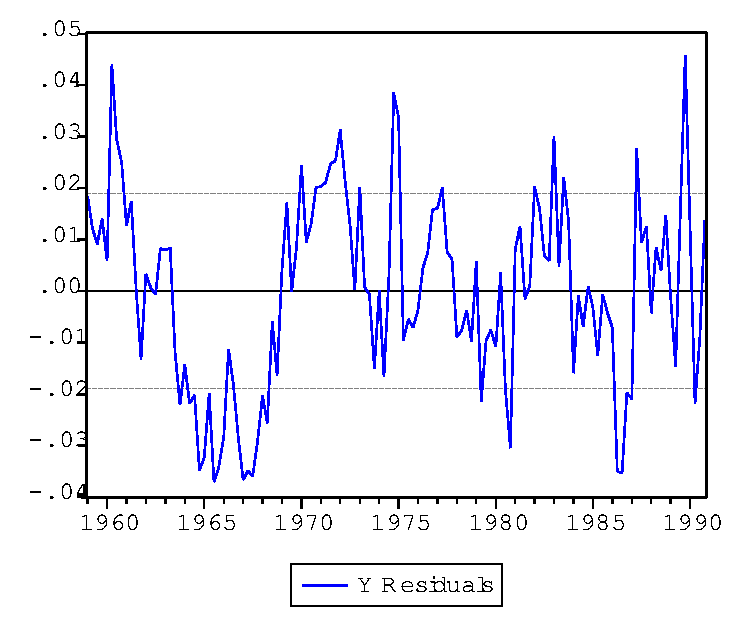
\includegraphics[scale=0.5,angle=0]{graph}
        \caption{Estimated residuals (2) from model XXX. ...}
        \label{Fig:Resids2}
    \end{center}
\end{figure}


% tables (not mandatory)
%\newpage
%\section{Tables}

\begin{table}[ht]
    \begin{center}
        {\footnotesize
        \begin{tabular}{l|cccccccccc}
        \hline \hline
                        & 3m    & 6m    & 1yr   & 2yr   & 3yr   & 5yr   & 7yr   & 10yr  & 12yr  & 15yr   \\
            \hline
                Mean   & 3.138 & 3.191 & 3.307 & 3.544 & 3.756 & 4.093 & 4.354 & 4.621 & 4.741 & 4.878  \\
                Median & 3.013 & 3.109 & 3.228 & 3.490 & 3.680 & 3.906 & 4.117 & 4.420 & 4.575 & 4.759  \\
                Min    & 1.984 & 1.950 & 1.956 & 2.010 & 2.240 & 2.615 & 2.850 & 3.120 & 3.250 & 3.395  \\
                Max    & 5.211 & 5.274 & 5.415 & 5.583 & 5.698 & 5.805 & 5.900 & 6.031 & 6.150 & 6.295  \\
                StD    & 0.915 & 0.919 & 0.935 & 0.910 & 0.876 & 0.825 & 0.803 & 0.776 & 0.768 & 0.762  \\
            \hline \hline
        \end{tabular}}
    \end{center}
    \caption{Detailed descriptive statistics of location and dispersion for
    2100 observed swap rates for the period from
    February 15, 1999 to March 2, 2007. Swap rates measured as 3.12 (instead of 0.0312).}
    \label{Tab:DescripStatsRawDataDetail}
\end{table}




% --------------------------------------------
% --- last page: Declaration of Authorship ---
% --------------------------------------------

%\newpage
%\thispagestyle{empty}
%%{\Large{\bf Declaration of Authorship}}\vspace{0.5cm}

\section*{Declaration of Authorship}

I hereby confirm that I have authored this Student Research Paper independently and without use of others than the indicated
sources. All passages which are literally or in general matter
taken out of publications or other sources are marked as such.
\vspace{1cm}

Berlin, \today \vspace{0.5cm}

Arne Binder



\end{document}
